\chapter{Deanonymization of transactions with network analysis} % Main chapter title

\label{Chapter03Clustering}

In this Chapter, we describe a novel network-level deanonymization attack on cryptocurrencies.\footnote{This Chapter is based on~\cite{Biryukov2019a, Biryukov2019b}. This work was partially supported by the Zcash Foundation through grant 2017Q4-24~\cite{Feher2017}.}
We show how a global passive adversary can cluster transactions that are likely to originate from the same node.
Such clusters can then be correlated with IP addresses.

Our method is based on analyzing the timings of transaction announcements.
Compared to~\cite{Biryukov2014} and~\cite{Koshy2014}, we do not only consider the first node that announces a transaction.
Our approach is more sophisticated.
We collect the data using servers on different continents to get a complete view of the network.
We then apply carefully chosen weight functions to transaction announcement timestamps.
We observe that transactions issued from the same node exhibit higher correlations between their weight vectors.
This technique allows us to cluster such transactions with high accuracy.
Our clustering method may act as a useful complement to transaction graph analysis based on blockchain data.

We test our method on Bitcoin and three alternative privacy-focused cryptocurrencies: Dash, Monero, and Zcash.
We are able to cluster our own transactions in Bitcoin and Zcash with high levels of precision and recall.
The cost of a full-scale attack on the Bitcoin mainnet is on the order of hundreds of US~dollars, which is feasible even for a low budget adversary.
Moreover, we unpack address advertisement messages (\texttt{addr}), which under certain assumptions may help link transaction clusters to IP addresses of the corresponding nodes.
We also demonstrate the applicability of our technique to the privacy-focused cryptocurrencies.
In particular, we demonstrate that we can cluster Zcash transactions that involve both transparent and shielded addresses.


\section{Transaction clustering with timing analysis}  \label{sec:Ch03Ourapproach}

We now describe our transaction clustering technique.

\subsection{Intuition}

Each transaction is initially introduced to the network by a single node -- the source.
The source first announces a transaction to its immediate neighbors -- its \textit{entry nodes}.
They, in turn, announce the transaction to their neighbors, and so forth.

Our goal is to divide all transactions into clusters, where each cluster corresponds to one source.
We connect to all nodes and log the timestamps of transaction announcements.
Intuitively, a peer that announces a transaction to us quickly is likely to be "close" to its source.
The \textit{first relayer heuristic} used in earlier attacks assumes that the first node to announce a transaction \textit{is} the source.
This heuristic is based on two assumptions:
\begin{enumerate}
	\item The attacker is directly connected to all nodes;
	\item All nodes announce a new transactions to all their neighbors as soon as they become aware of it.
\end{enumerate}
Both assumptions do not fully hold in practice.
First, not all nodes accept incoming connections.
Therefore, if a source node does not accept incoming connections, the attacker would learn about its transactions from other nodes.
Second, cryptocurrencies use deliberate \textit{broadcast randomization} methods to break the latter assumption.
In particular, Bitcoin uses diffusion, whereas Zcash uses trickling (see Section~\ref{sec:BitcoinP2PProtocol} for details).

Our method overcomes the limitations of the first relayer heuristic.
We exploit the fact that transactions from the same source are announced through the same set of entry nodes.
For each transaction, we construct \textit{weight vectors}.
Each element of a vector corresponds to a node\footnote{We identify nodes by their IP~addresses} that announced at least one transaction to us.
We assign decreasing non-zero weights to the first $N$~nodes that announced the transaction to us.
All others receive a zero weight.
We expect to observe a higher correlation between the vectors for transaction that come from the same source, compared to transaction that do not.

As an example, consider a source with eight entry nodes $p_1, \dots, p_8$.
It announces three transactions: $tx_1$, $tx_2$, and~$tx_3$.
Ideally, all transactions are broadcast via the same subset of the entry nodes, for instance, $p_1$, $p_2$, and~$p_3$.
In that case, the weight vectors would be easy to correlate: they all would have non-zero elements at positions $1$, $2$, and~$3$.
But due to broadcast randomization, the following scenario is more typical: $tx_1$ is relayed via $p_{\{1,2,3\}}$, $tx_2$ via $p_{\{3,4,5\}}$, and~$tx_3$ via $p_{\{5,6,7\}}$.
Based on weight vectors, considering that those are sparse, our technique detects the relationship between the transactions even in this case.
The correlation between $tx_1$ and~$tx_2$ and between $tx_2$ and~$tx_3$ would be noticeable.
This allows us to reveal not only the relationship between these two transaction pairs, but also among all three transactions.

This technique is also applicable for transactions originating from a light client.
In that case, a cluster represents transactions from multiple clients connected to the same full node.


\subsection{Weight functions and clustering}

Let $tx$ be a transaction.
Let $p^{tx} = [p^{tx}_1, p^{tx}_2, \dots, p^{tx}_N]$ be the vector of the first $N$~IP addresses which relayed $tx$ to us.
Let $t^{tx} = [t^{tx}_1, t^{tx}_2, \dots, t^{tx}_N]$ be the vector of the corresponding \textit{relative} timestamps.
A \textit{relative} timestamp is defined as $t = t^{abs}_i - t^{abs}_0$, where $t_{abs}^i$ is the absolute time (Unix timestamp) when we received transaction $tx_i$ (i.e.,~we subtract the timestamp of the first announcement of each transaction from all its announcements).
For each $p^{tx}_i \in p^{tx}$, we assign a parameterized weight as follows:

\[
w_k(p^{tx}_i) = e^{-(t^{tx}_i/k)^2}
\]

The weight function is chosen to reflect the decreasing importance of every next announcement.
$p_1$ is assigned the maximum weight of~$1.0$ ($t_1=0$ by definition).
Other nodes receive lower weights.
Our experiments show that this function family yields better clustering (compared to $1/(kt)$ and~$e^{-kt}$).
The intuition is that it gives higher weights to a certain window depending on $k$, while exponentially decreasing outside of it.
Moreover, window size is adjusted for each vector.

For each $p^{tx}$, we want to use such $w_k$ that gives sufficient variance among the weight values.
Weights quickly fall to nearly zero if $k$ is too low and stay close to one if $k$ is high.
Let $t^{tx}_{med}$ be the median value in~$t^{tx}$.
We choose $k^{tx}_{opt}$ such that the weight of~$t^{tx}_{med}$ is equal to~$0.5$:

\[
k^{tx}_{opt} = \frac{t^{tx}_{med}}{\sqrt{-\ln(0.5)}}
\]

This choice of~$k$ distributes the weights for any $t^{tx}$: they neither stay close to one nor quickly fall to zero (see examples in Figure~\ref{fig:weight}).
\begin{figure}
	\centering
	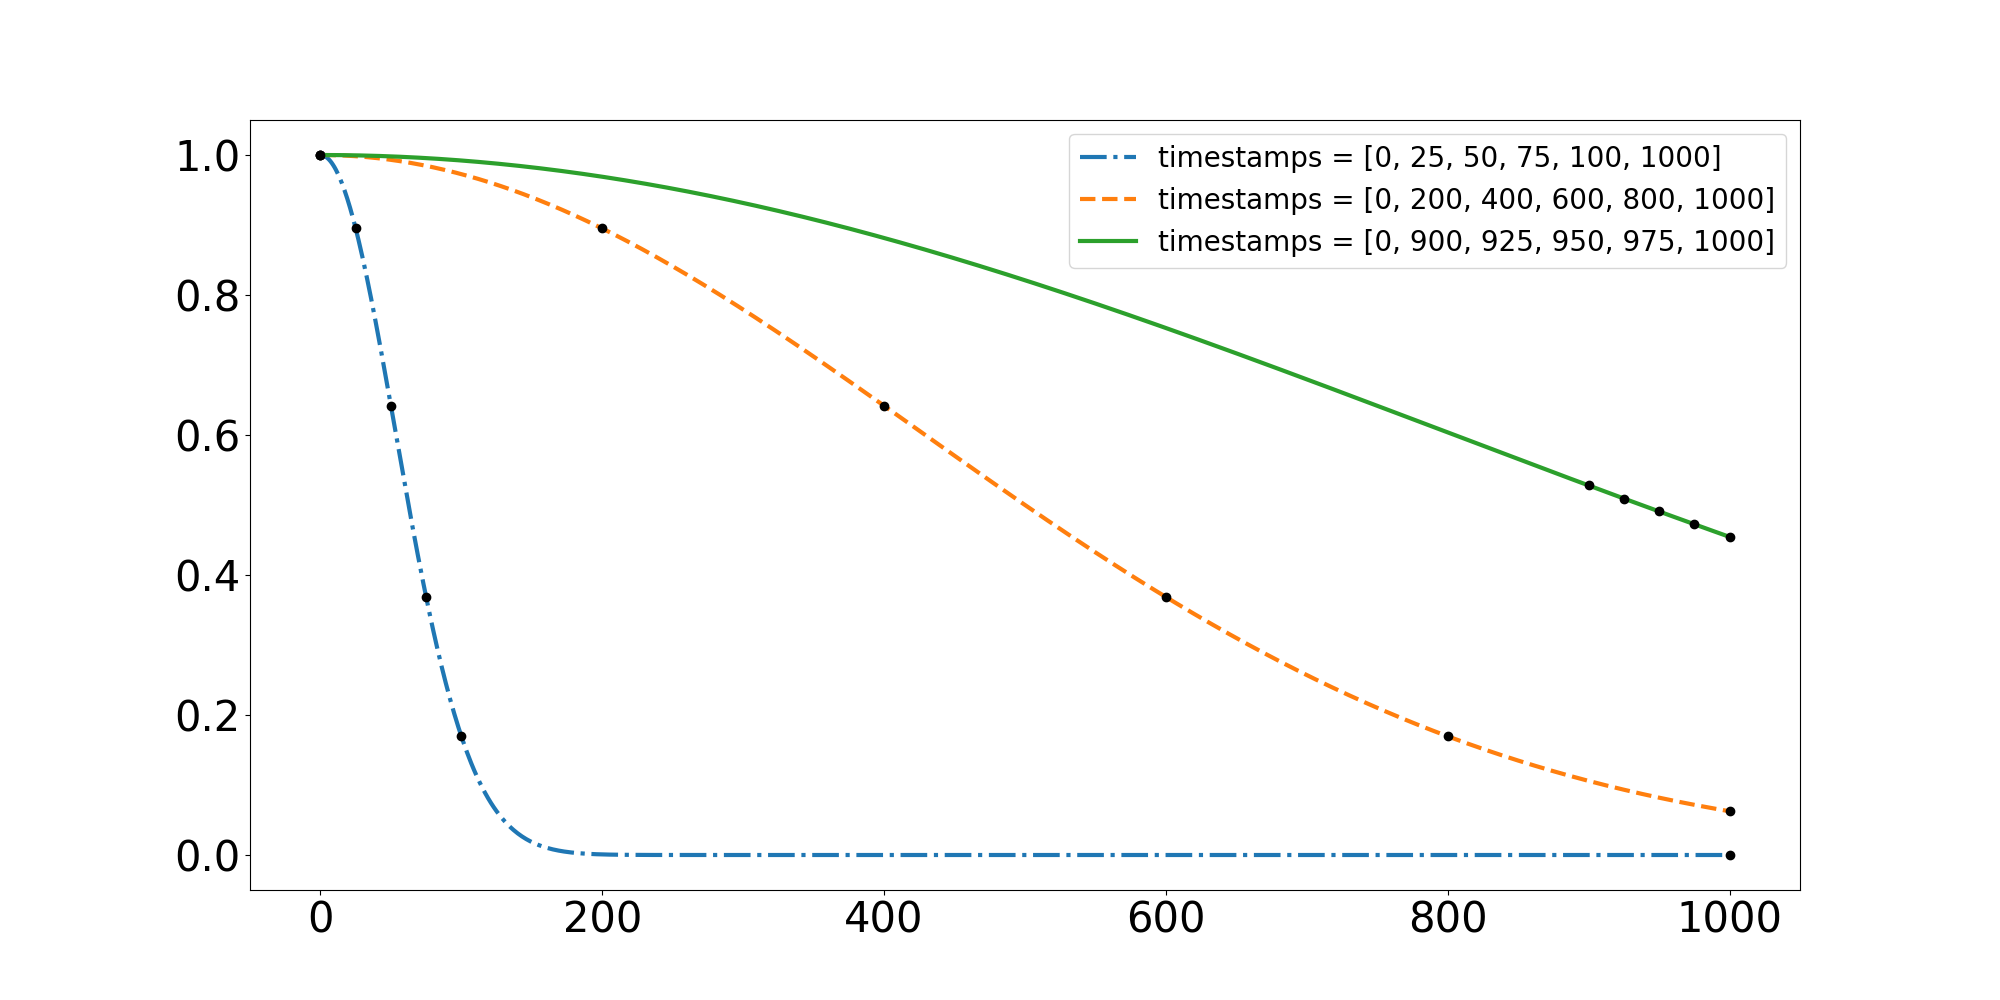
\includegraphics[width=\columnwidth]{weight-function-example.png}
	\caption{Weight functions for three timestamp vectors.}
	\label{fig:weight}
\end{figure}
For each transaction, we evaluate the vector of weights:

\[
w^{tx} = w_{k^{tx}_{opt}}(t^{tx})
\]

Let $X$ be the set of all transactions we consider.
Let $P$ be the set of IP addresses of nodes which appeared in at least one of~$p$ vectors in $X$:

\[
P = \bigcup\limits_{tx \in X} p^{tx}
\]

We define an extended weight vector $v_{tx}$ for each~$tx$ by setting the weight of nodes in $P \backslash p^{tx}$ to zero and sort the values in the weight vectors w.~r.~t.~the alphabetical order of~$P$.
We then calculate a matrix where an element in $i$-th row and~$j$-th column is the Pearson correlation of the extended weight vectors $v_{tx_i}$ and~$v_{tx_j}$.
This matrix can supposedly be transformed into a block-diagonal matrix with blocks (clusters) corresponding to transaction sources.

To reveal the clusters, we use spectral co-clustering~\cite{Dhillon2001} implemented in the Python \texttt{sklearn.cluster.bicluster} module~\cite{scikitlearn2018}.
Given an input matrix $A$, the algorithm preprocesses it as follows:

\[
A_n = R^{1/2}AC^{-1/2}
\]

Where $R$ is the diagonal matrix with entry $i$ equal to $\sum_{j} A_{ij}$, and~$C$ is the diagonal matrix with entry $j$ equal to $\sum_{i} A_{ij}$.

The singular value decomposition of~$A$ provides the partitions of rows and columns: $A_{n}=U \Sigma V^{T}$.
The $l$ = $\lceil \log_2 k \rceil$ singular vectors provide the partitioning information.
Let $U$ be a matrix with columns $u_2,\dots,u_{l+1}$, and similarly for $V$.
Then $Z$ is defined as:

\[
Z = 
\begin{bmatrix}
R^{-1/2} & U \\
C^{-1/2} & V
\end{bmatrix}
\]

The rows of~$Z$ are clustered using the k-means algorithm.


\subsection{Measuring clustering quality}

We use the Rand score as an external metric of clustering quality (see~\cite{Amigo2009}, Section~4.2).
The Rand score operates on \textit{pairs} of elements and reflects the proportion of "right decisions" regarding whether to put a pair of transactions into the same cluster or different clusters.

$SS$,~$SD$,~$DS$, and~$DD$ are numbers of transaction pairs defined as follows:
\begin{itemize}
	\item SS: same cluster, same category (two of our transactions in the same cluster);\footnote{In our case, there are only two categories: "our" and "foreign" transactions.}
	\item SD: same cluster, different category (our and foreign transactions in the same cluster);
	\item DS: different cluster, same category (two of our transactions in different clusters);
	\item DD: different cluster, different category (our and foreign transactions in different clusters).
\end{itemize}

Note that this assessment only considers clusters with "our" transactions, because we do not know whether any two "foreign" transactions should have been assigned to the same cluster:

\[
R = \frac{SS + DD}{SS + SD + DS + DD}
\]

We further modify this metric by parameterizing it with the minimal number of our transactions in a cluster required to consider this cluster in the calculation.
In our experiments, we only consider clusters with at least two of our transactions.
With no such threshold, large clusters with one of our transactions disproportionately increase $DD$ and bring the score close to $1.0$, which does not reflect the subjective amount of information an adversary acquires.

\subsection{Measuring the degree of deanonymization}

To estimate the success rate of the attack, we use a quality score based on the \textit{anonymity degree}~\cite{Diaz2002}.
The anonymity degree is designed to measure the amount of information an attacker gains compared to perfect anonymity.
Consider a transaction the attacker has captured.
The goal is to assign a probability that is originates from~$S_{control}$.
Initially, all transactions are assigned equal probabilities (perfect anonymity).
Then the attacker re-assigns these probabilities with respect to clustering.
The anonymity degree reflects the amount of information the attacker gains by doing so.

Let $p_i$ be the probability that a transaction~$i$ originates from~$S_{control}$.
$N$ is the total number of transactions.
The entropy is calculated as:

\[
H = -\sum_{i=1}^N p_i log_2(p_i)
\]

The maximum entropy is:

\[
H_M = log_2(N)
\]

The anonymity degree is defined as:

\[
d = \frac{H}{H_M}
\]


Our goal is to cluster transactions originating from one target source $S_{control}$.
Our of~$N$~captured transactions, $n$ were issued from~$S_{control}$.
We know $k$~of them.
For each transaction~$i$, the a priori probability of having originated from~$S_{control}$ is $p_i = n / N$.

We then uses the clustering algorithm to improve these probabilities.
This is done in two steps.
First, all captured transactions are divided into clusters.
However, there is no guarantee that only one cluster corresponds to~$S_{control}$.
The clustering algorithm may divide the control transactions into two clusters (together with other, mistakenly included transactions).
To account for this, each cluster is assigned a \textit{weight} that reflects how likely is this cluster to represent $S_{control}$.
For example, consider $10$~transactions $t_0, \dots, t_9$.
Five of them, $t_0, \dots, t_4$, were announced from the target source~$S_{control}$.
Let us assume that the clustering algorithm divides the transactions into them into three clusters as follows: $c_a = \{t_0, t_1, t_2, t_3\}, c_b = \{t_4, t_5, t_6, t_7\}, c_c = \{t_8, t_9\}$.
Let us assume that the attacker knows that $t_0$ and~$t_4$ actually originate from~$S_{control}$.
The attacker therefore assigns a weight of~$0.5$ to clusters $c_a$ and~$c_b$, and a weight of~$0$ to cluster~$c_c$.
Therefore, the total "probability weight" of all transactions from $S_{control}$ is distributed evenly among transactions from $c_a$ and~$c_b$ ($t_0, \dots, t_7$).
Note that the true distribution is $1$ for transactions $t_0, \dots, t_4$ and~$0$ for all others.

Finally, the \textit{adjusted} anonymity degree accounts for cluster weights.
We calculate the median square error~$e$ between the vectors of probabilities $p_i$ derived by the attacker and the true probabilities.
The adjusted anonymity degree is defined as follows:

\[
d_{adj} = 1 - (1 - e) \times (1 - d)
\]

Consider two edge case examples.
If $e = 0$ (the attacker correctly guessed the~$S_{control}$ cluster), $d_{adj} = d$.
If $e = 1$ (the attacker's cluster weights do not at all reflect the reality), $d_{adj} = 1$ (the system retains full anonymity).

The assumptions of our model have their limitations.
Our method depends on a user issuing a series of transactions in a relatively short time window of several minutes (up to an hour), through the same set of entry nodes (i.e.,~the same session).
If a user re-launches the software, their transactions issued before and after this event would not be linkable by our technique.
%While this scenario may not be prevalent, it may gain popularity in the future, as cryptocurrencies gain broader adoption and at least partially solve the scalability issues.


\section{Implementation details}

We used a modified Bitcoin network probing tool \texttt{bcclient}~\cite{Pustogarov2017} to maintain parallel connections to peers and log incoming messages.
The tool is relatively easy to adapt for usage with Dash and Zcash, which mostly inherit Bitcoin's networking layer.
We re-compiled \texttt{bcclient} with modified constants (port numbers, protocol magic bytes, DNS seeder addresses).
For Monero, which is not based on the Bitcoin~Core codebase, we modified the full node reference implementation (\texttt{monerod}).
We added the required logging and disabled the built-in limits on the total bandwidth as well as artificial delays between network requests.

For each transaction announcement, we logged the transaction hash, the IP which announced it to us, and the timestamp of this event.
Our method does not need full transaction data.
Therefore, we only logged \texttt{inv} messages, and never continue with the \texttt{getdata} -- \texttt{tx} exchange.
For selected experiments on Bitcoin testnet, we also log \texttt{addr} messages.
This allows us to infer the set of most probable IP addresses that correspond to each transaction cluster.

We use Python scripts to extract the data from the log, save it in a more compact JSON format, analyze it, and visualize the results.

\section{Experimental evaluation}

The outline of our experiment is as follows:

\begin{enumerate}
	\item collect a fresh list of live peers;
	\item establish a number of parallel connections to them;
	\item launch the listening node and start logging the timestamps of the received \texttt{inv} and \texttt{addr} messages;
	\item launch two nodes $S_{learn}$ and~$S_{control}$;%, so that their initial \texttt{addr} advertisements are logged;
	\item issue two series of transactions: the learning set from~$S_{learn}$ and the control set from~$S_{control}$;
	\item for each considered number of first propagations, calculate the transaction correlation matrix;
	\item run the clustering algorithm with various assumed average number of transactions per cluster;
	\item choose the best clustering by Rand score based on the "learning" set;
	\item in the best clustering, assign the cluster weights proportionally to the distribution of~$k$~known transactions from~$S_{control}$;
	\item assign zero probability of being in~$S_{control}$ to transactions from~$S_{learn}$;
	\item re-distribute the probability weight among transactions in each cluster;
	\item calculate the final adjusted anonymity score;
	\item re-arrange the clusters such that high correlation values are close to the main diagonal;
	\item visualize the results.
\end{enumerate}

We visualize the results using heatmaps.
We assign a color to each element of the matrix, where each row and each column represents an announced transaction.
The color of the square at the intersection of the~$i$-th row and~$j$-th column represent the correlation of weight vectors of~$i$-th and~$j$-th transactions.
Darker colors represent higher correlation.
Note the the heatmap is diagonally symmetric by definition.
Black squares along the main diagonal reflect the fact that each weight vector is perfectly correlated with itself.

We permute rows and columns such that the highly correlated elements are close to the main diagonal.
We expect such permutation to cause the matrix to exhibit a block-diagonal structure.
Blocks of highly correlated elements grouped along the main diagonal represent the clusters.
In the figures below, ticks along the axes indicate our transaction from the control set.


\subsection{Results for desktop wallets}

We evaluate our method by clustering our own transactions in Bitcoin (testnet and mainnet) and Zcash.
For these experiments, we log the traffic for $15$~minutes.
For Dash and Monero, we ran the clustering algorithm without calculating the anonymity degree.
We obtained clearly visible clusters, which indicated that our approach is applicable for these cryptocurrencies as well.

All linkage experiments were done on our own transactions and when possible on the testnets.
The experiments on the Bitcoin mainnet deliberately did not attempt to occupy all connection slots, and operated only on a subset of~$1000$~nodes (out of approximately $10\,000$~nodes reachable at any given time~\cite{Bitnodes}).

In this section, we refer to the node that logs the incoming messages as the \textit{listener}.
Following the terminology of~\cite{Biryukov2014}, we refer to peers that accept incoming connections as \textit{servers}.

% California: experiment-1541509693
% Tokyo: experiment-1541511845
% Frankfurt: experiment-1541513977
% 3-experiment: experiment-1541516997
\begin{table*}[!t]
	\normalsize
	\caption{Summary of the experimental results on Bitcoin testnet and Zcash.}
	\centering
	\begin{tabular}{|l|l|c|c|c|c|c|}
		\hline
		Network & Listener & Anon\@. deg. & Servers & Avg free slots & Tx \texttt{inv}s & \texttt{addr}s \\
		\hline
		Bitcoin test & California & $0.83$ & $1141$ & $64$ & $139$ & $402$ \\
		Bitcoin test & Tokyo & $0.80$ & $1128$ & $64$ & $193$ & $414$ \\
		Bitcoin test & Frankfurt & $0.72$ & $1137$ & $64$ & $172$ & $403$ \\
		Bitcoin test & combined & $0.63$ & $1154$ & $63$ & $250$ & $1321$ \\
		Bitcoin main & Frankfurt & $0.88$ & $1000$* & $25$* & $3238$ & $11\,300$ \\
		Zcash & Frankfurt & $0.86$ & $206$ & $36$ & $62$ & $1086$ \\
		\hline
	\end{tabular}
	\label{tab:results}
\end{table*}

\subsubsection{Bitcoin testnet}

We performed four experiments on the Bitcoin testnet using different listener locations.
In three experiments, we used single listeners in one of the three geographical locations: Frankfurt (Germany), Tokyo (Japan), and North California (the US).
In the fourth experiment, we used the aforementioned listeners simultaneously.
We divided the list of live peers into three equal parts and distributed them among the three listeners.
Each listener connected only to the peers from its part of the list.
We then merged the three log files.
The goal of the fourth experiment was to measure the advantage an adversary may gain from using geographically distributed servers.

The listeners attempted to occupy up to establish $117$~connections to each assigned peer.
All test transactions were issued from computers located in Luxembourg.
We issued two sets of test transactions (the learning and the control sets) containing $30$~transactions each.
We denote $10$~transactions out of the control set as "known" to estimate the anonymity degree.

The results are presented in Table~\ref{tab:results} and Figures~\ref{fig:bitcoin-testnet-california},~\ref{fig:bitcoin-testnet-tokyo},~\ref{fig:bitcoin-testnet-frankfurt}, and~\ref{fig:bitcoin-testnet-combined}.
The "*"~sign in the table indicates the experiments where we only connected to a subset of available nodes.

The number of live peers collected by each of the listeners is very close.
This indicates that we do obtain a complete view of the network.
Note also that the number of received transactions varies little between experiments, whereas the number of \texttt{addr} messages is significantly higher in the experiment with three listeners.
This confirms our hypothesis that \texttt{addr} messages propagate through the network more slowly than transactions.
The number of average available slots is independent of the location of the listener.

The anonymity degree calculated on our own transactions indicates a substantial loss of privacy.
The joint experiment with three geographically distributed listeners gained the best results with an anonymity degree of~$0.63$.
Out of the three single-listener experiments, the anonymity degree is lower (i.e.,~better for the attacker) in the Frankfurt experiment.
This may be explained by the fact that the test transactions were issued from a much closer location than in the other experiments.


\begin{figure*}
	\centering
	\begin{minipage}{0.5\textwidth}
		\centering
		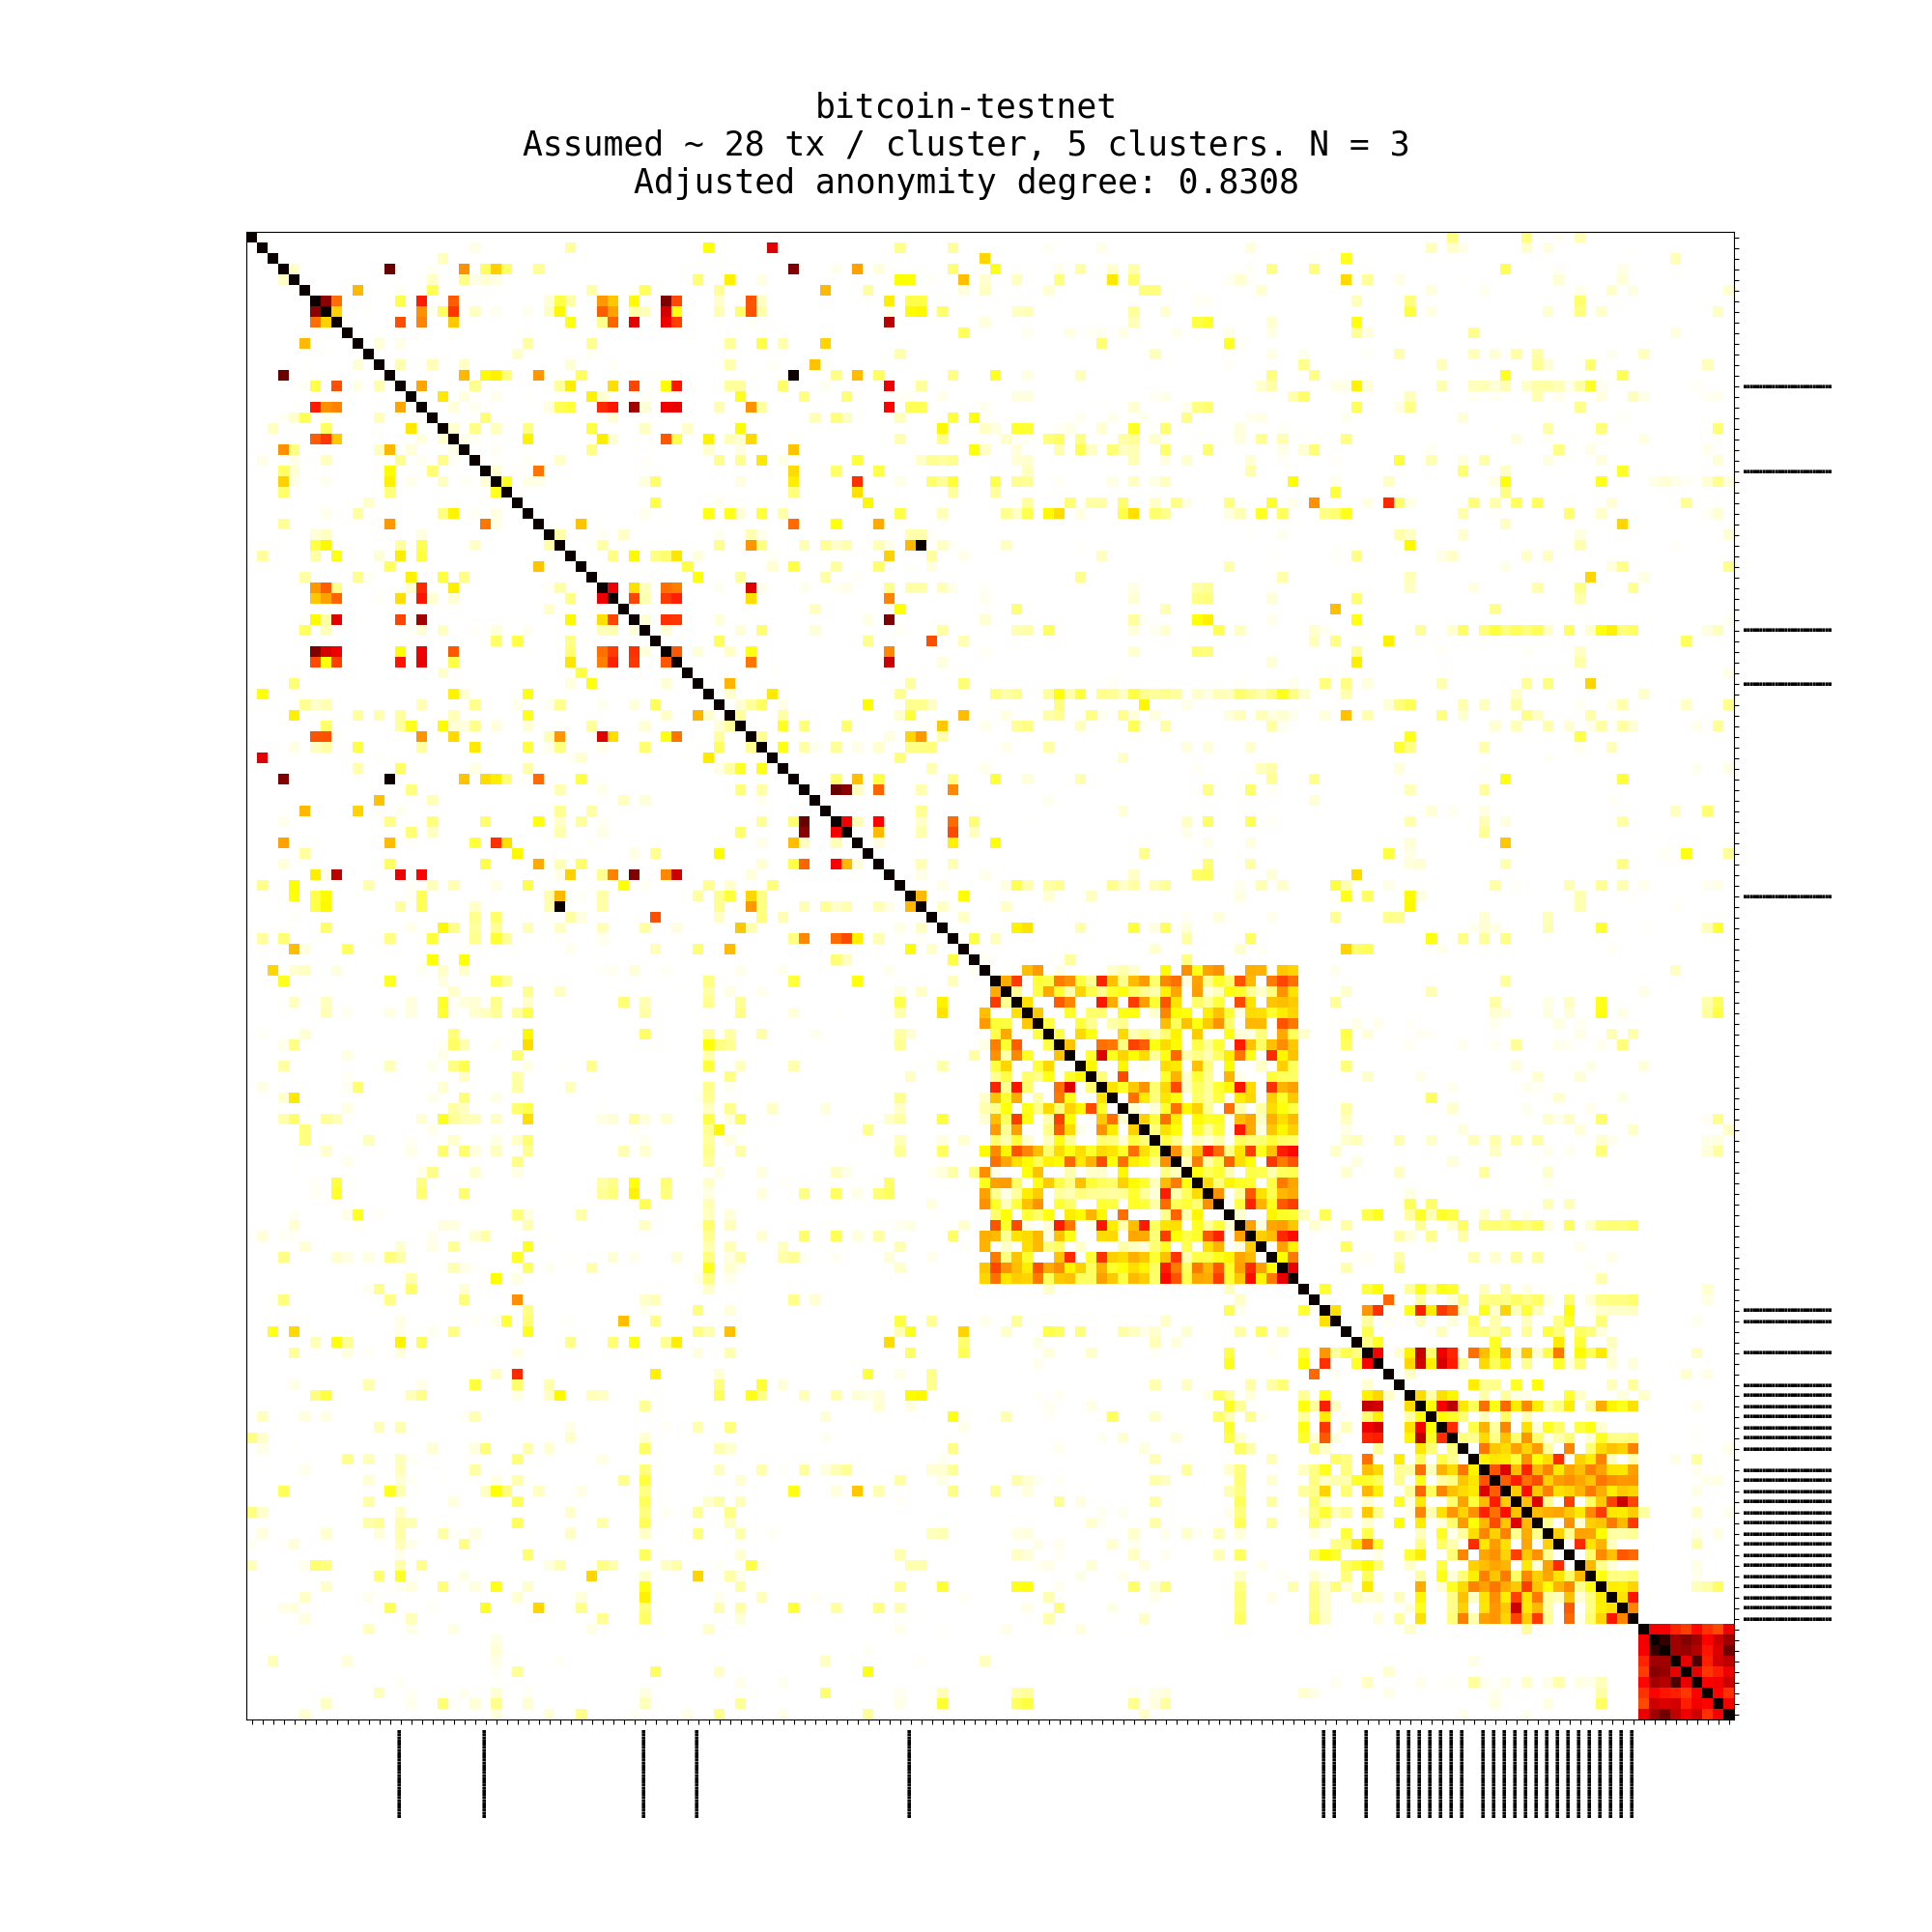
\includegraphics[width=\columnwidth]{bitcoin-testnet-1541509693-California.png}
		\caption{Transaction clustering for Bitcoin testnet (listener in California).}
		\label{fig:bitcoin-testnet-california}
	\end{minipage}\hfill
	\begin{minipage}{0.5\textwidth}
		\centering
		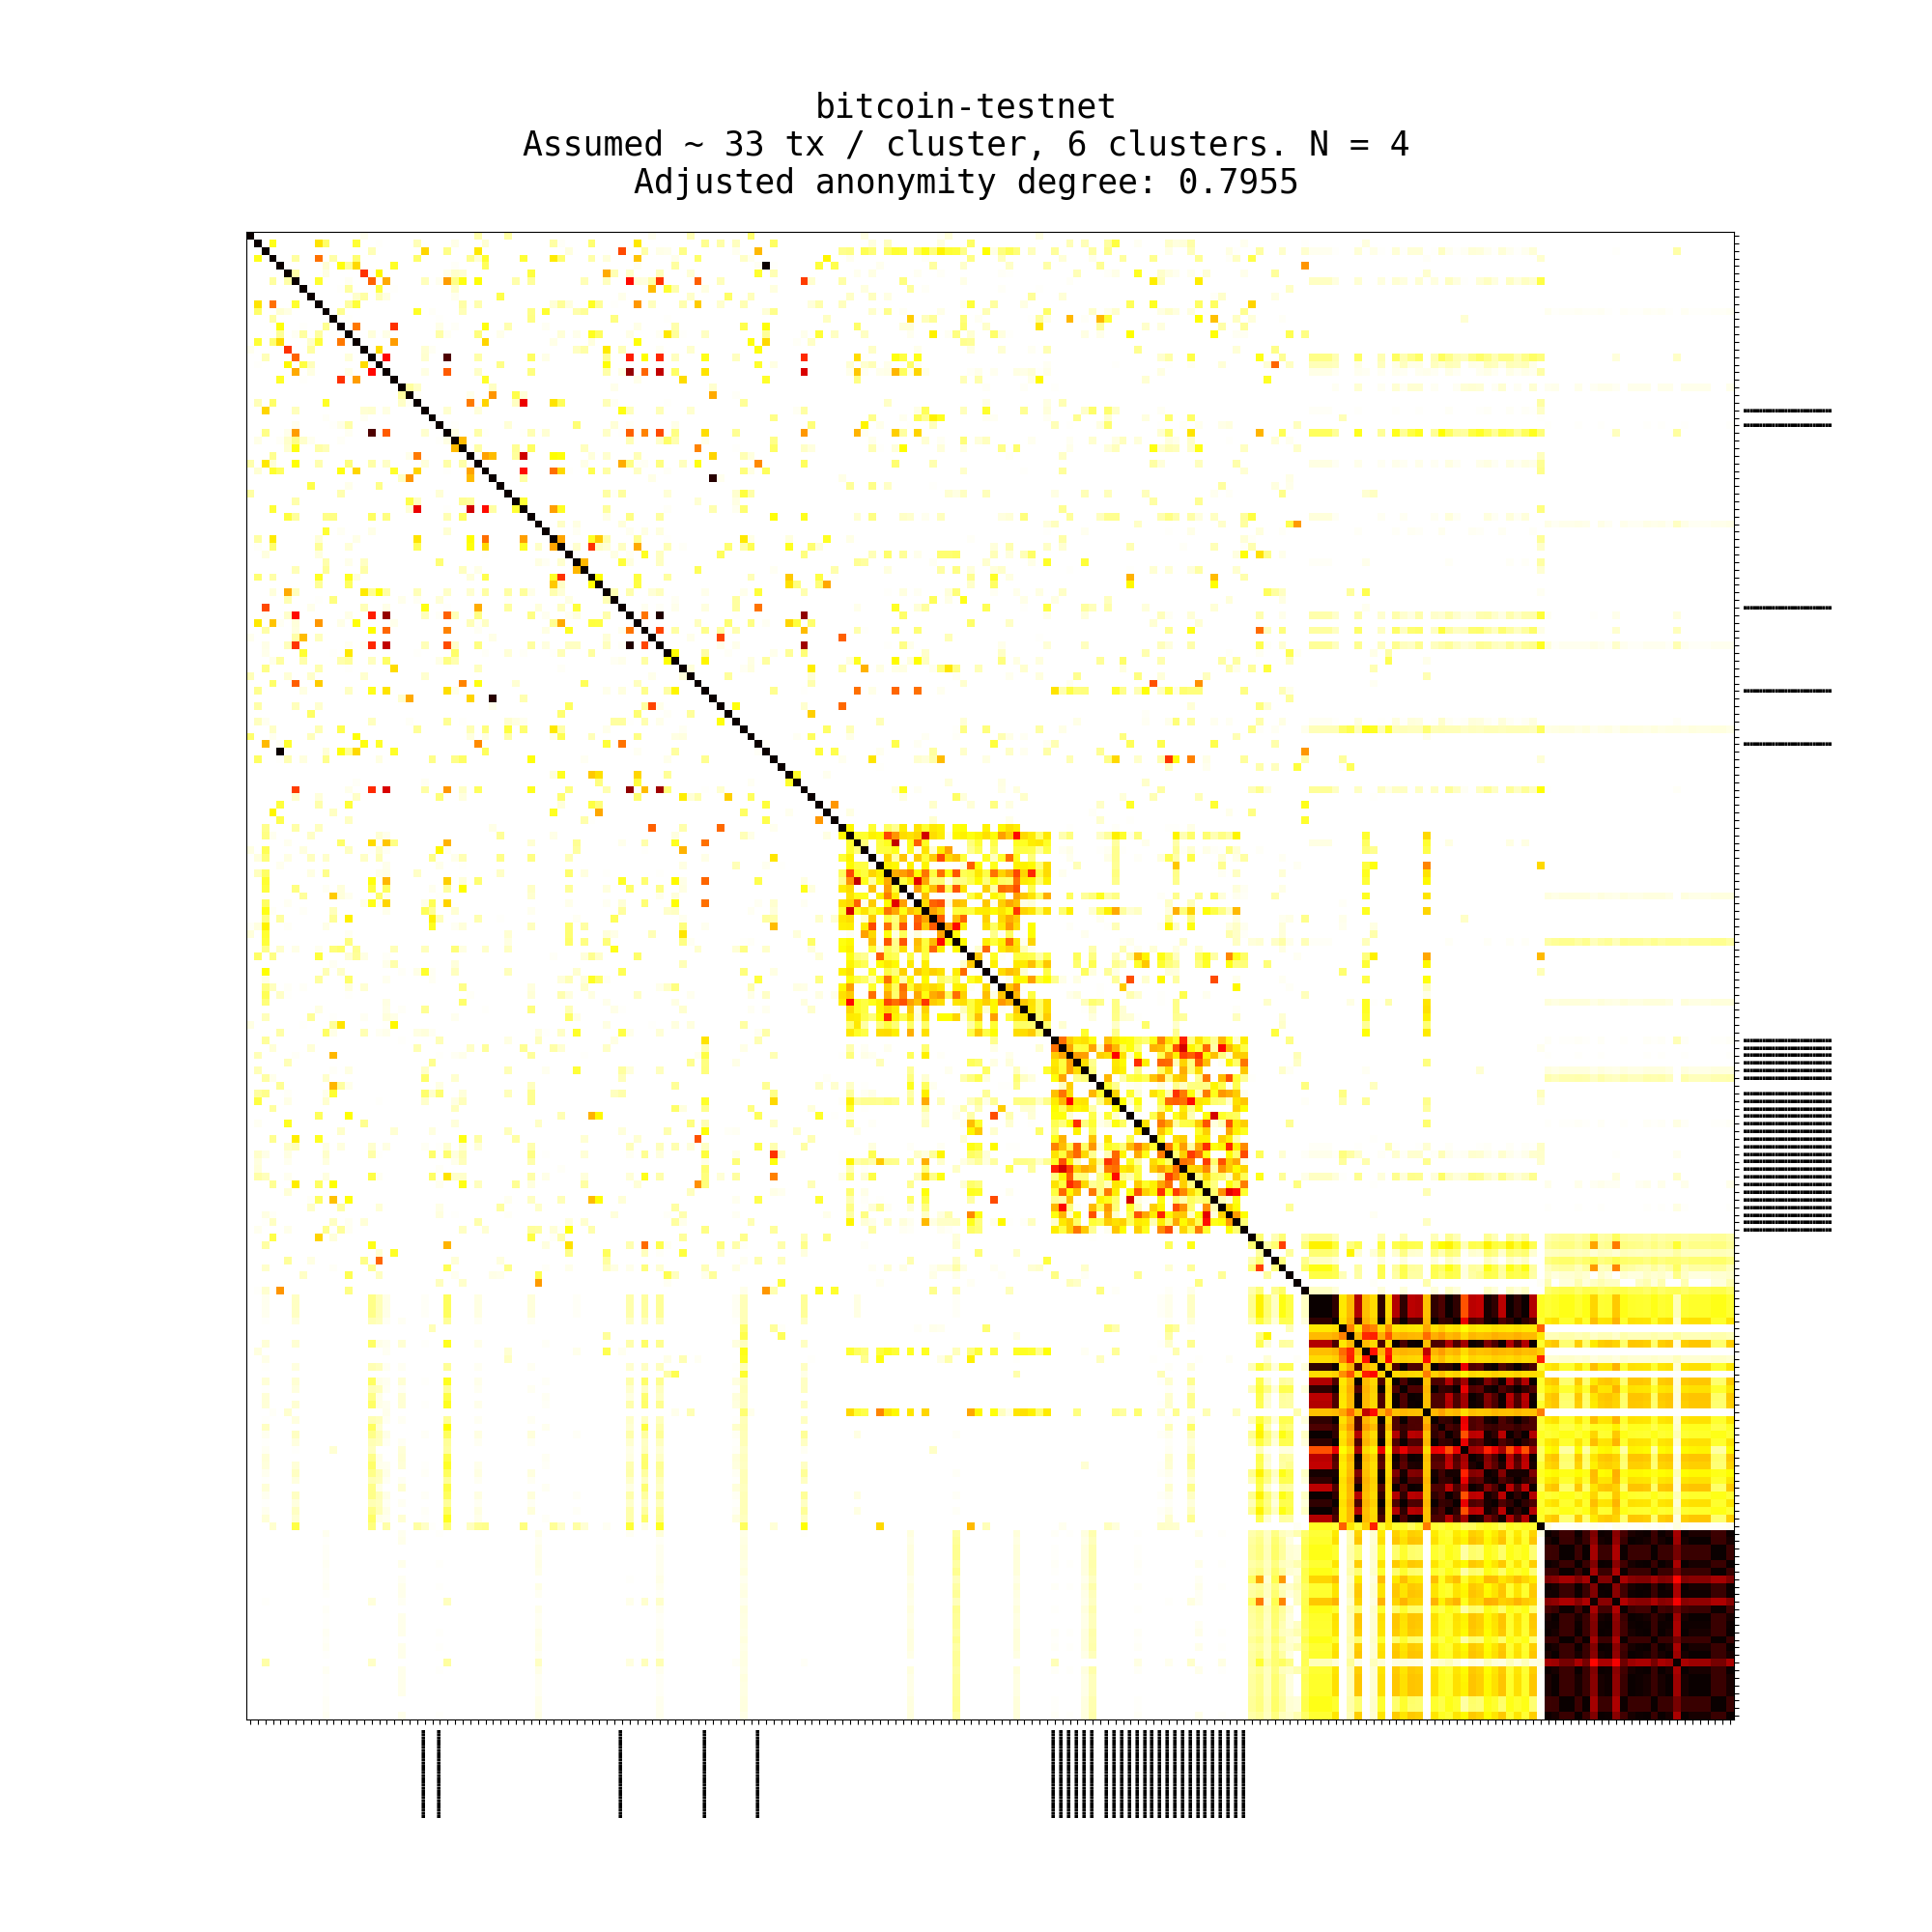
\includegraphics[width=\columnwidth]{bitcoin-testnet-1541511845-Tokyo.png}
		\caption{Transaction clustering for Bitcoin testnet (listener in Tokyo).}
		\label{fig:bitcoin-testnet-tokyo}
	\end{minipage}\hfill
\end{figure*}

\begin{figure*}
	\centering
	\begin{minipage}{0.5\textwidth}
		\centering
		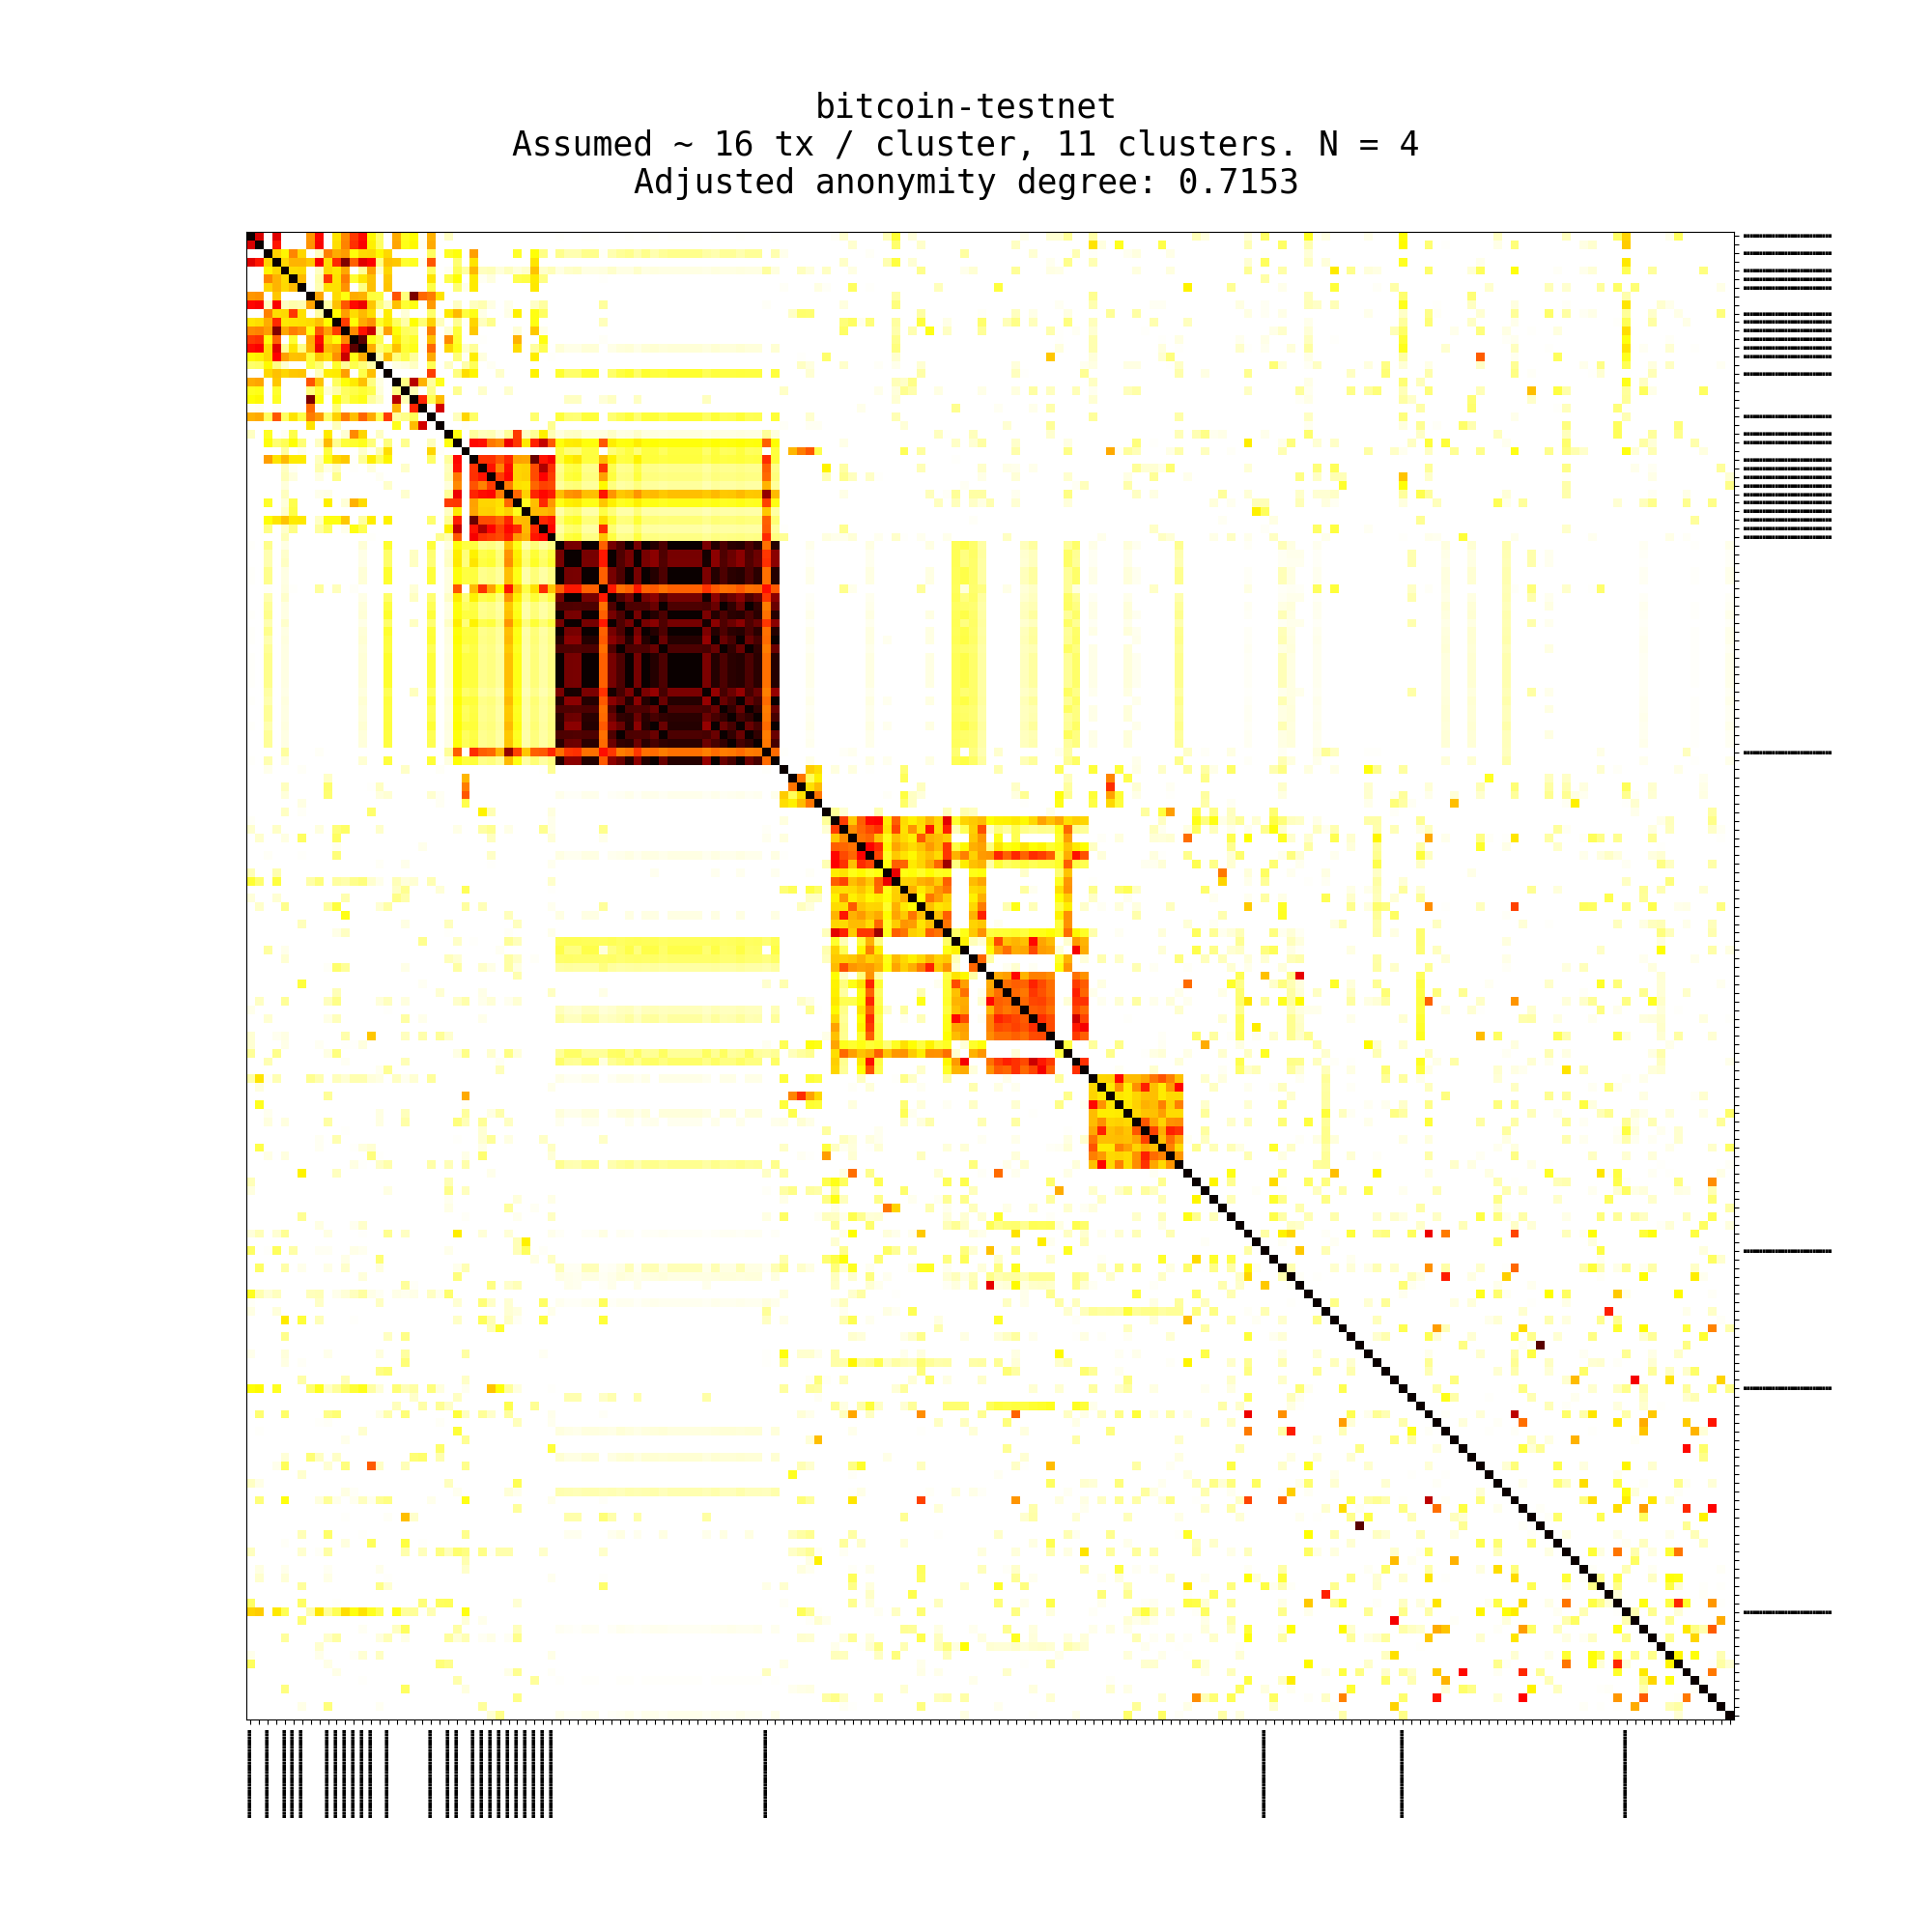
\includegraphics[width=\columnwidth]{bitcoin-testnet-1541513977-Frankfurt.png}
		\caption{Transaction clustering for Bitcoin testnet (listener in Frankfurt).}
		\label{fig:bitcoin-testnet-frankfurt}
	\end{minipage}\hfill
	\begin{minipage}{0.5\textwidth}
		\centering
		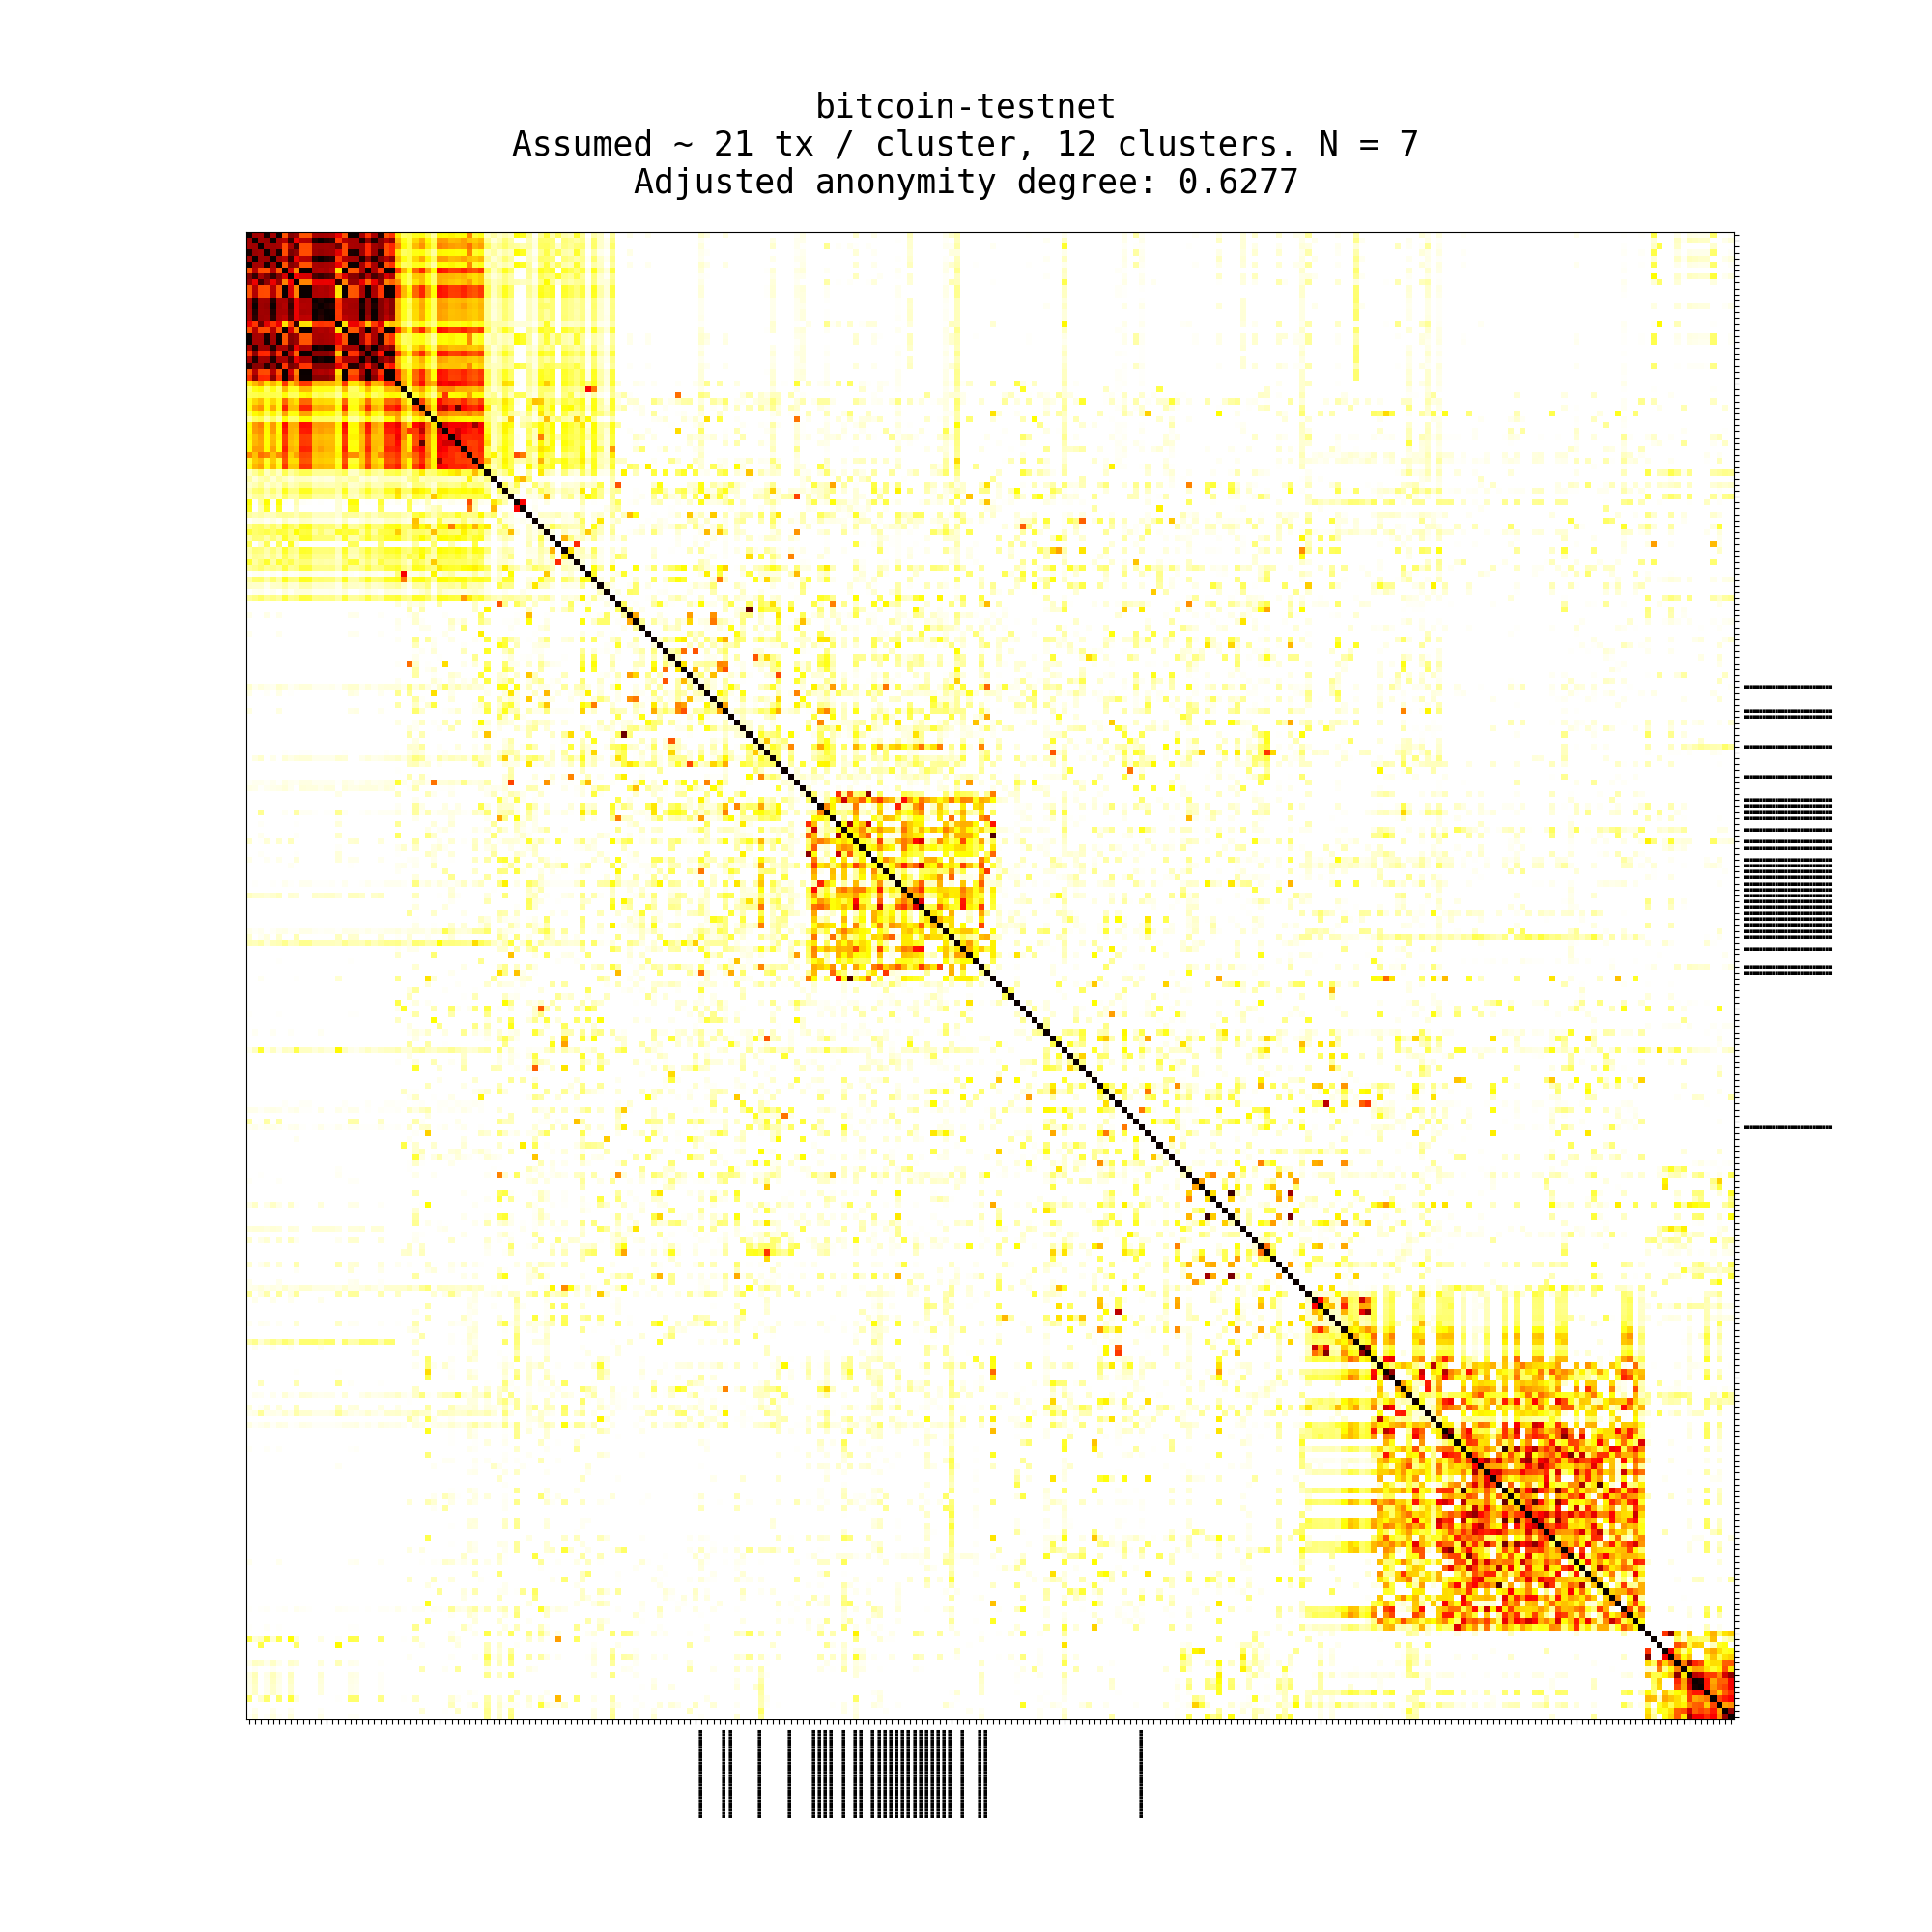
\includegraphics[width=\columnwidth]{bitcoin-testnet-1541516997-combined.png}
		\caption{Transaction clustering for Bitcoin testnet (combined listeners).}
		\label{fig:bitcoin-testnet-combined}
	\end{minipage}\hfill
\end{figure*}


\paragraph{Estimating the original IP}

We use the \texttt{addr} messages to determine (with some level of precision) the IP of the node which issued the transactions in the control group.
In our experiments, we first launch the listener, and only then launch the issuing nodes.
This means that the listener captures the \texttt{addr} messages issued by the issuing nodes during bootstrapping.
Address messages propagate through the network more slowly than transactions and are periodically re-broadcast.
A listener can distinguish between \texttt{addr} messages of recently joined nodes and re-broadcasts of older \texttt{addr} messages.
If only one or two nodes announce an IP address, which is most often the case, we assume it is a re-broadcast.
If more nodes announce an IP address, we assume that the node has just joined the network or is re-advertising its IP.
% after an approximately 24~hours delay.

Our idea is to leverage the \texttt{addr} messages as follows.
For each cluster, we determine the IPs of the most "important" nodes, i.e.,~nodes we assume are entry nodes of the transaction source.
For each transaction in the cluster, we sum up the weights of all IPs which relayed it to us.
We assume the top $10\%$~of most weighted IPs to be the entry nodes.
The intuition is that the entry nodes are among the first to relay \texttt{addr} messages from the original source.
Therefore, we assume that an \texttt{addr} message relayed by a set of IPs which substantially intersects with the entry nodes contains the IP address of the source of the cluster.

We applied this heuristic to the Bitcoin testnet experiments.
We considered the clusters that mostly consisted of control transactions.
We then derived the list of "likely" source IP addresses as per the heuristic described above.
In three out of four experiments, the true IP address was among the top five most likely source IPs.
This result indicates that an adversary can narrow down the search for the source IP address to only a handful of IPs.
This gives the attacker valuable information, such as the approximate geographical location of the victim.

\subsubsection{Bitcoin mainnet}

For Bitcoin mainnet, we performed one experiment with a listener located in Frankfurt.
We used learning and control transaction sets of~$20$~transactions each.
Five transactions from the control set were assumed "known" for anonymity degree calculation.

The results are presented in Table~\ref{tab:results} and Figures~\ref{fig:bitcoin-mainnet} and~\ref{fig:zcash}.
The transactions also exhibit the "clustering" behavior, though the anonymity decrease is weaker.
This may be caused by multiple factors.
First, Bitcoin mainnet is substantially larger than other networks we considered.
A higher number of transactions in Bitcoin constitutes a larger anonymity set.
Second, Bitcoin nodes have fewer free slots, and often limit the number of slots one IP can occupy.
This decreases the probability that our listener would be among the first nodes to receive a new transaction.
Third, we only established up to $50$~connections to $1000$~peers to avoid disrupting the network, and due to resource constraints.

\begin{figure*}
	\centering
	\begin{minipage}{0.5\textwidth}
		\centering
		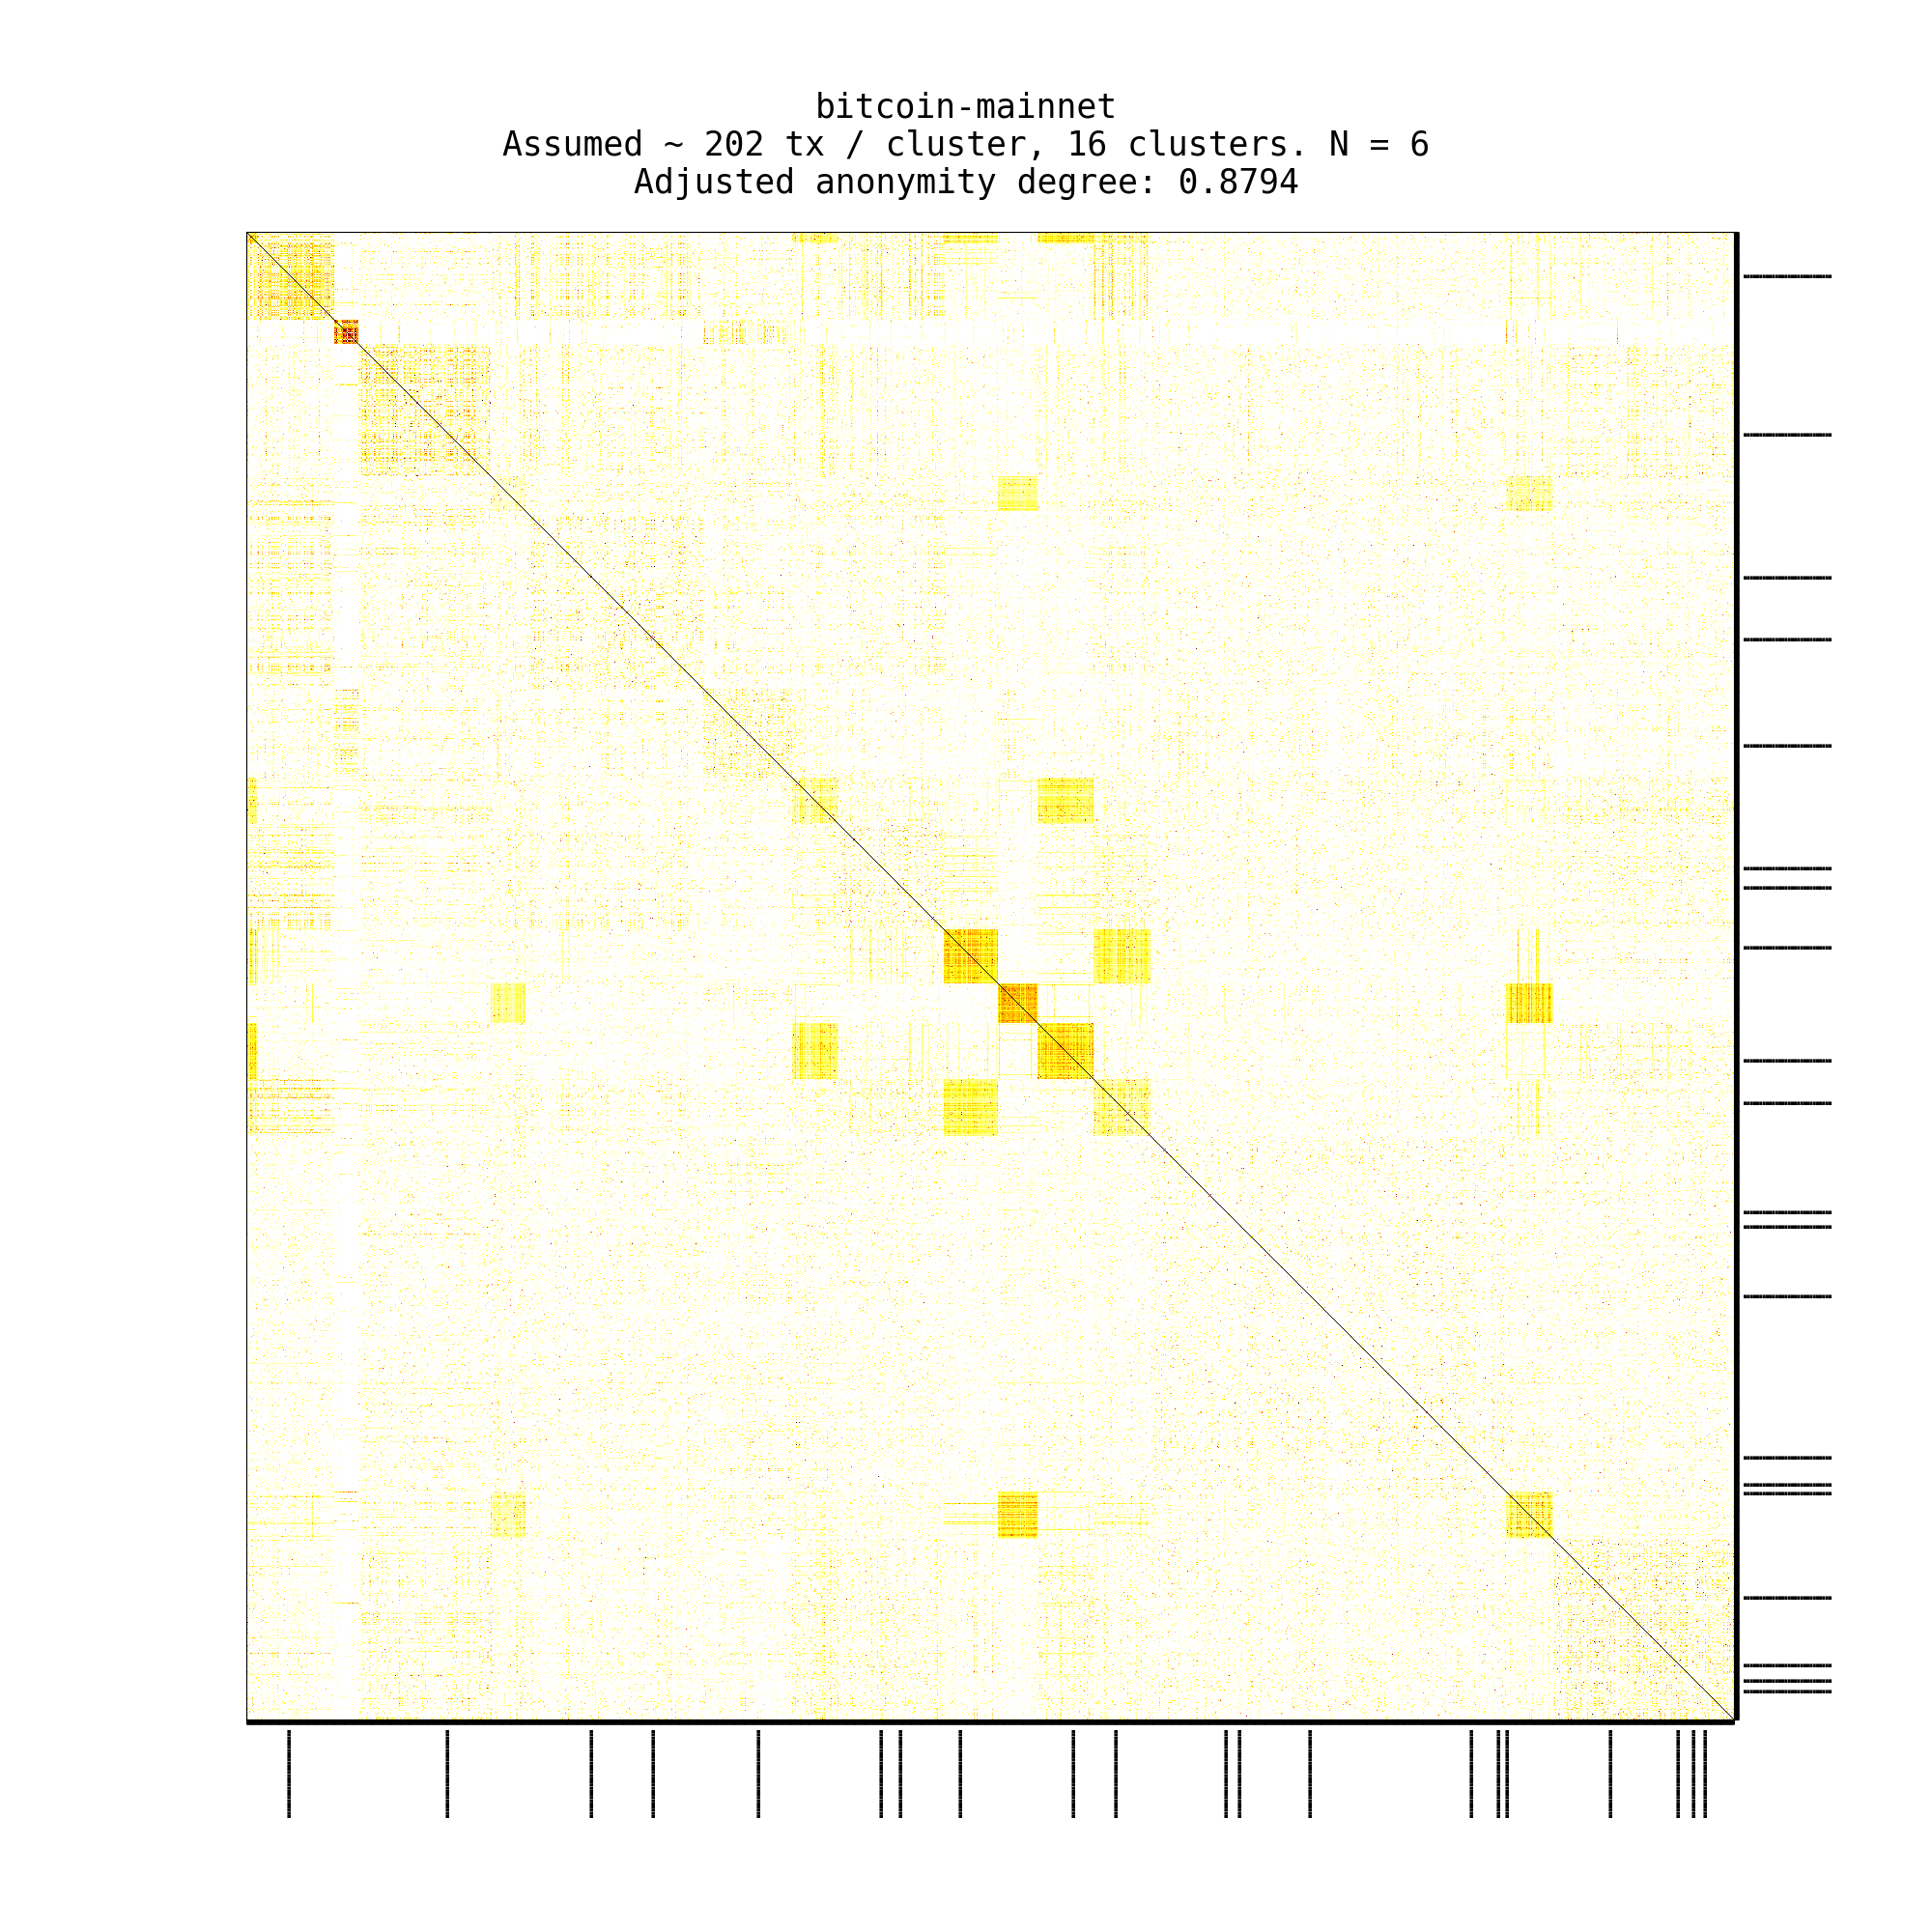
\includegraphics[width=\columnwidth]{bitcoin-mainnet-1542054034-fig-correlations-202-txcl-006-N-Rand-best.png}
		\caption{Transaction clustering for Bitcoin mainnet.}
		\label{fig:bitcoin-mainnet}
	\end{minipage}\hfill
	\begin{minipage}{0.5\textwidth}
		\centering
		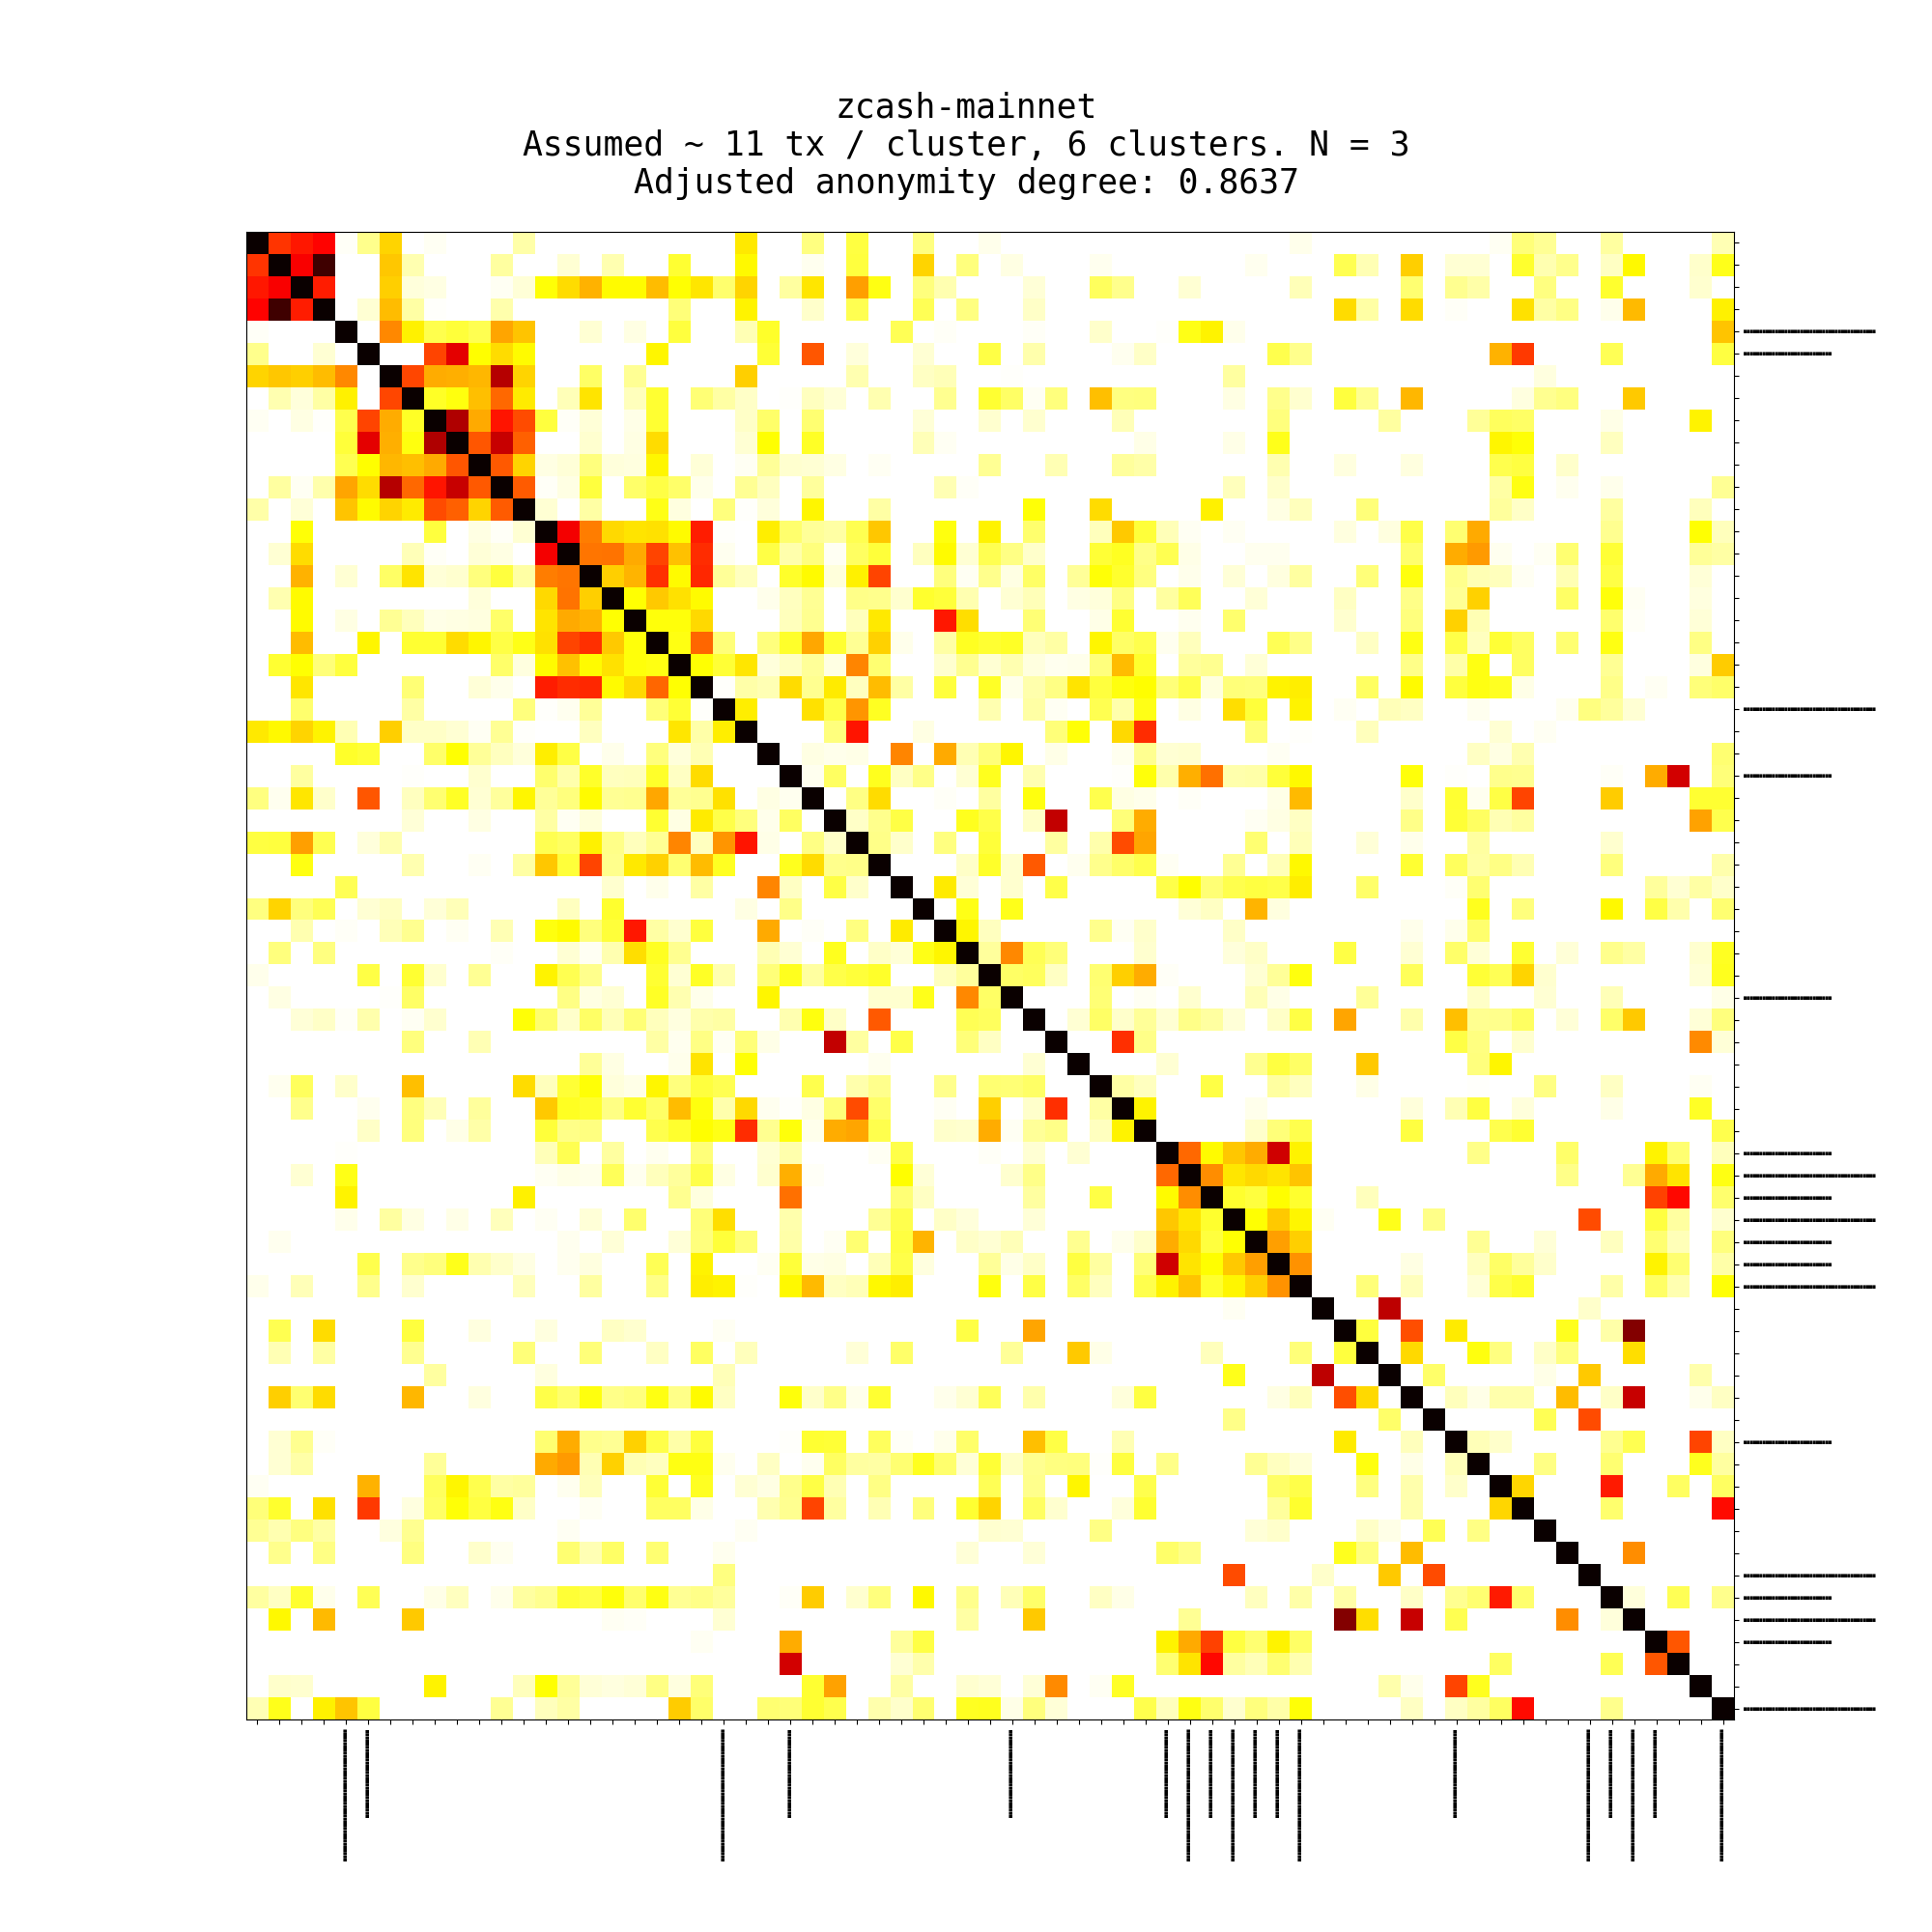
\includegraphics[width=\columnwidth]{zcash-mainnet-1541938472-Frankfurt.png}
		\caption{Transaction clustering for Zcash.}
		\label{fig:zcash}
	\end{minipage}\hfill
\end{figure*}

\subsubsection{Zcash}

Zcash is based on the codebase of Bitcoin~Core as of November~2015.\footnote{Bitcoin~Core~version~0.11.2 (commit~7e27892).}
As of time of our experiments (2018), Zcash user trickling as broadcast randomization technique, while Bitcoin had switched to diffusion.

Zcash does not provide privacy by default.
Zero-knowledge proofs are used only in transactions involving \textit{shielded} addresses~\cite{Kappos2018}.
The majority of transactions happen between \textit{transparent} addresses and have no additional privacy-preserving mechanisms compared to Bitcoin.

For the Zcash mainnet, we performed one experiment with a listener located in Frankfurt.
The learning and control sets consisted of~$20$ and~$18$~transactions respectively.
Eight~out of~$18$~control transactions were shielded (from a t-address to a z-address).
We used $6$~control transactions as "known" for anonymity degree estimation.

The results are presented in Figures~\ref{fig:bitcoin-mainnet} and~\ref{fig:zcash}.
Note that our attack does does not take into account transaction content or type.
Consequently, our method applied for Zcash allows clustering transactions involving both transparent and shielded addresses.
Transactions from the control set that involve shielded addresses are marked with longer ticks in the figure.

%The Zcash network is much smaller than the Bitcoin testnet.
We notice that Zcash peers offer far fewer free connection slots on average: $36$~compared to $64$~on Bitcoin testnet (see Figures~\ref{fig:free-slots-bitcoin} and~\ref{fig:free-slots-zcash}).
A relatively high number of servers only provided our listener with up to ten connection slots.
This may indicate a larger share of "protected" nodes, i.e.,~nodes which are configured (using firewalls or other network-level mechanisms) to only provide a limited number of connections to each IP\@.
Note than a resourceful adversary may overcome this limitation by purchasing IP addresses from a cloud provider.

\begin{figure*}
	\centering
	\begin{minipage}{0.5\textwidth}
		\centering
		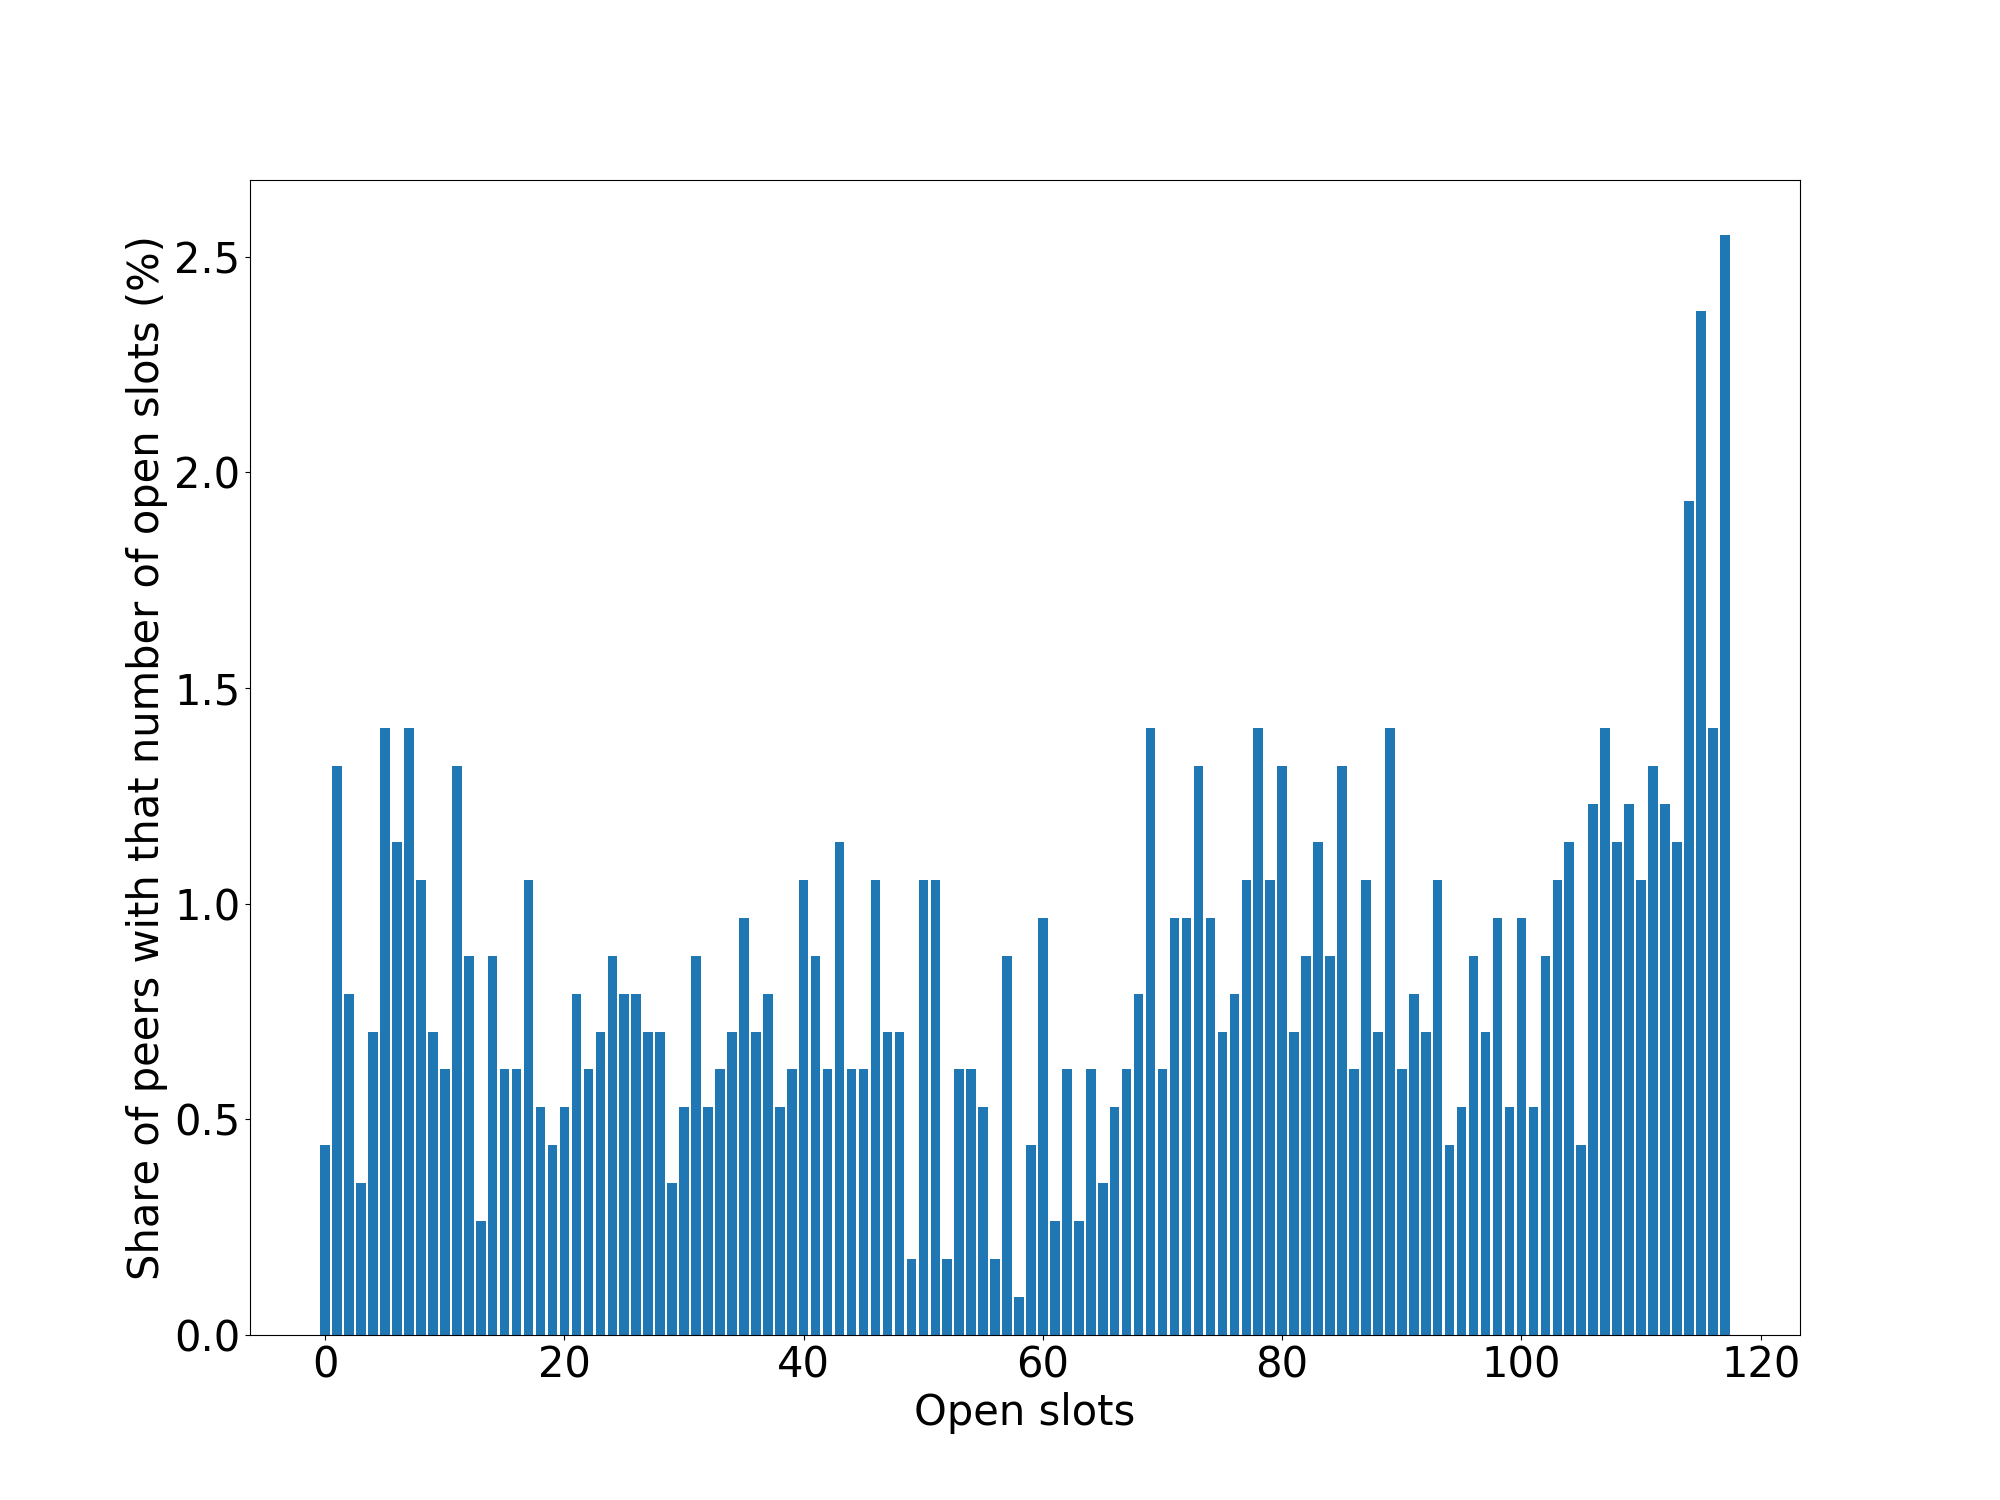
\includegraphics[width=\columnwidth]{bitcoin-testnet-1541513977-conn-max-histogram.png}
		\caption{Free connection slots: Bitcoin testnet.}
		\label{fig:free-slots-bitcoin}
	\end{minipage}\hfill
	\begin{minipage}{0.5\textwidth}
		\centering
		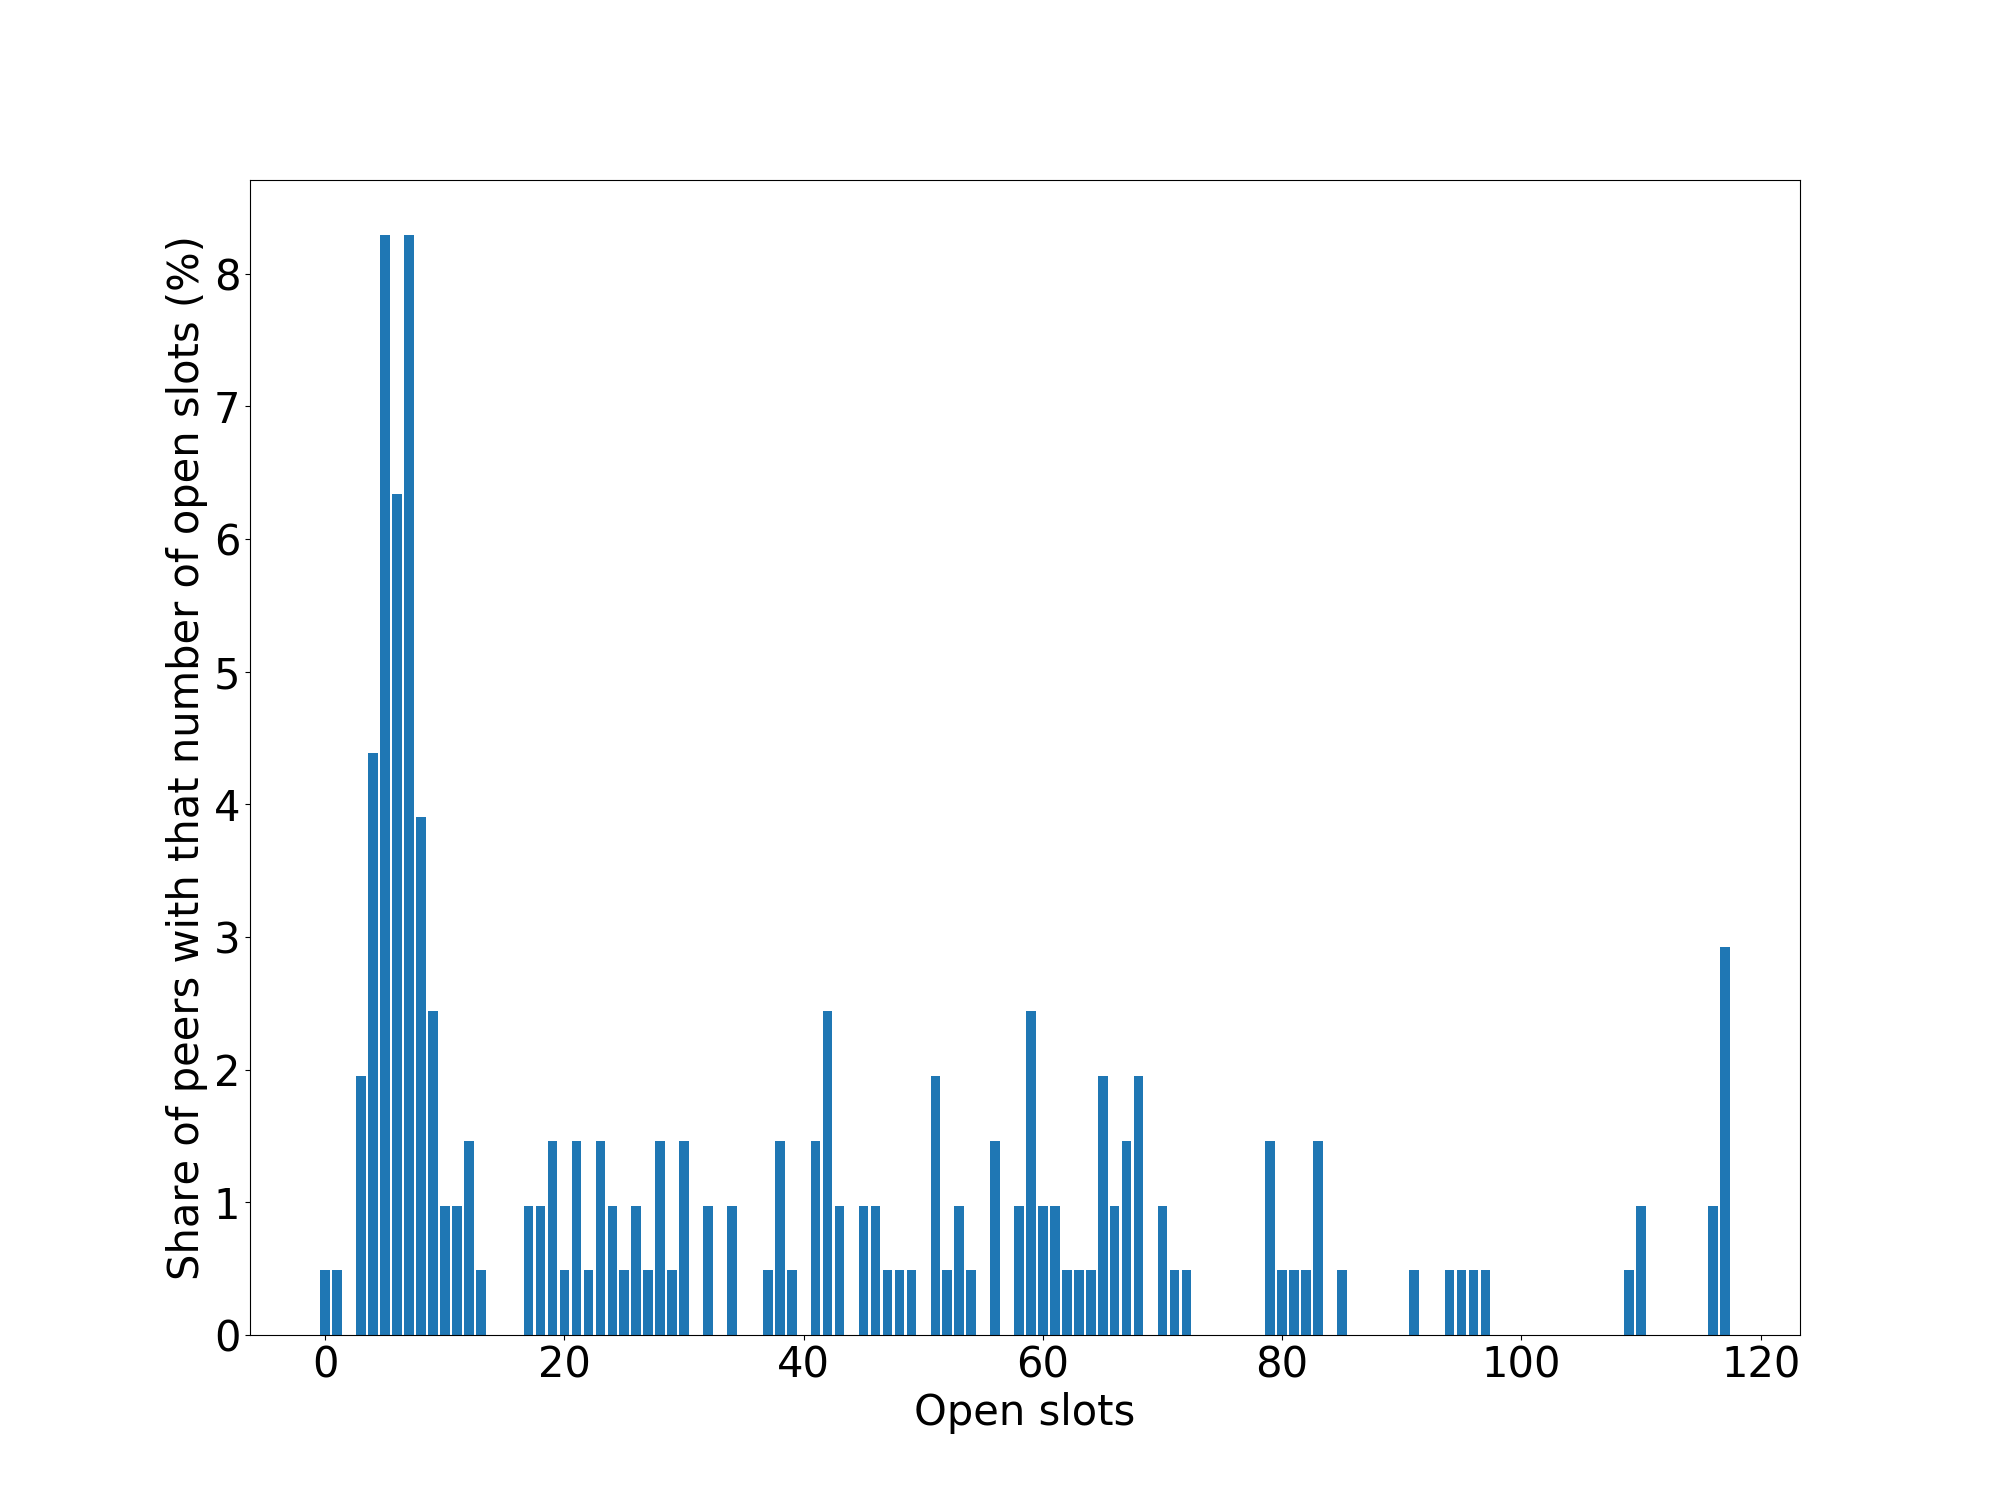
\includegraphics[width=\columnwidth]{zcash-mainnet-1541938472-conn-max-histogram.png}
		\caption{Free connection slots: Zcash mainnet.}
		\label{fig:free-slots-zcash}
	\end{minipage}\hfill
\end{figure*}


\subsubsection{Dash}

Dash is also based on the codebase of Bitcoin~Core and inherits the basics of its networking protocol.
Dash ported uses diffusion broadcast randomization mechanism from Bitcoin.
The Dash networking protocol is however substantially more complex.
In addition to the message types present in Bitcoin, Dash contains $22$~new ones, mostly used for managing the masternode network~\cite{Schinzel2015}.
Masternode-related tasks include periodic pings to check whether masternodes are online, managing transaction mixing, voting for governance proposals, etc.
Our tool is not yet adapted for handling Dash-specific messages.

In our experiment, we connected to $500$~out of~$3065$~Dash nodes chosen at random, asking for $30$~connection slots.
During $15$-minutes, we received $12$~transaction inventory messages and~$396$~Dash-specific messages.

\begin{figure*}
	\centering
	\begin{minipage}{0.5\textwidth}
		\centering
		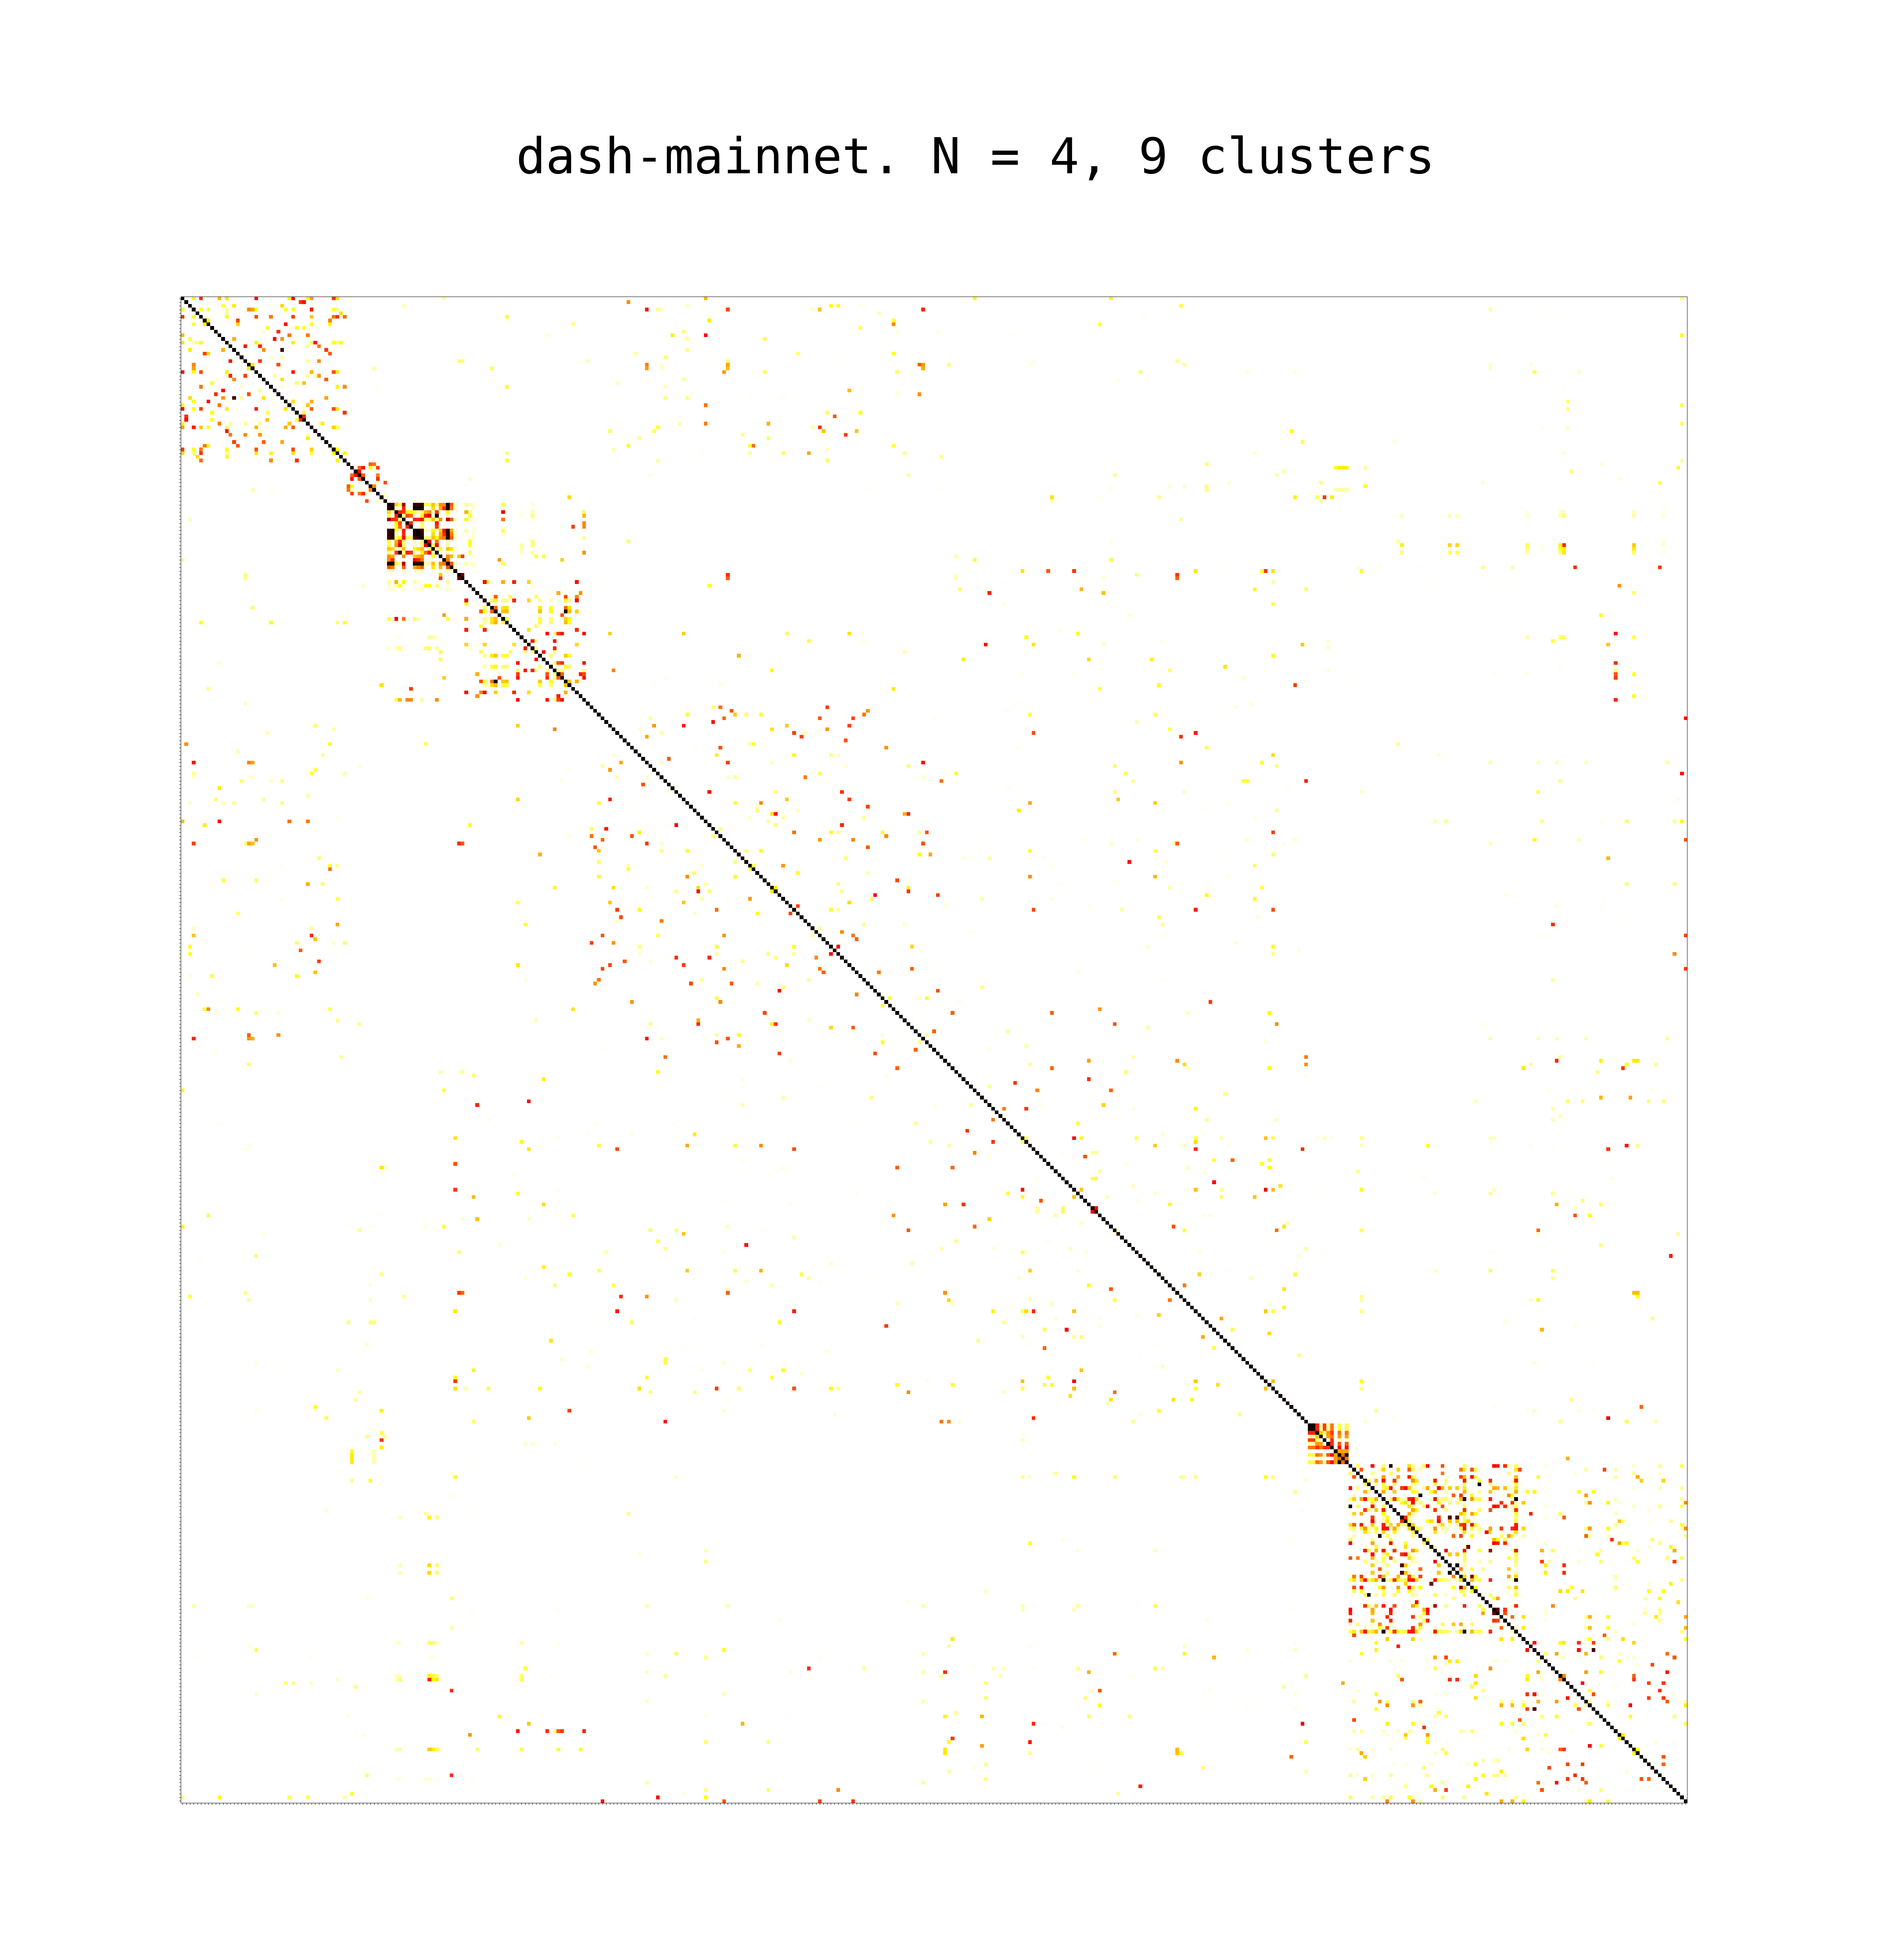
\includegraphics[width=\columnwidth]{dash-mainnet-1531510768-all.png}
		\caption{Transaction clustering for Dash (messages and transactions).}
		\label{fig:dash-all}
	\end{minipage}\hfill
	\begin{minipage}{0.5\textwidth}
		\centering
		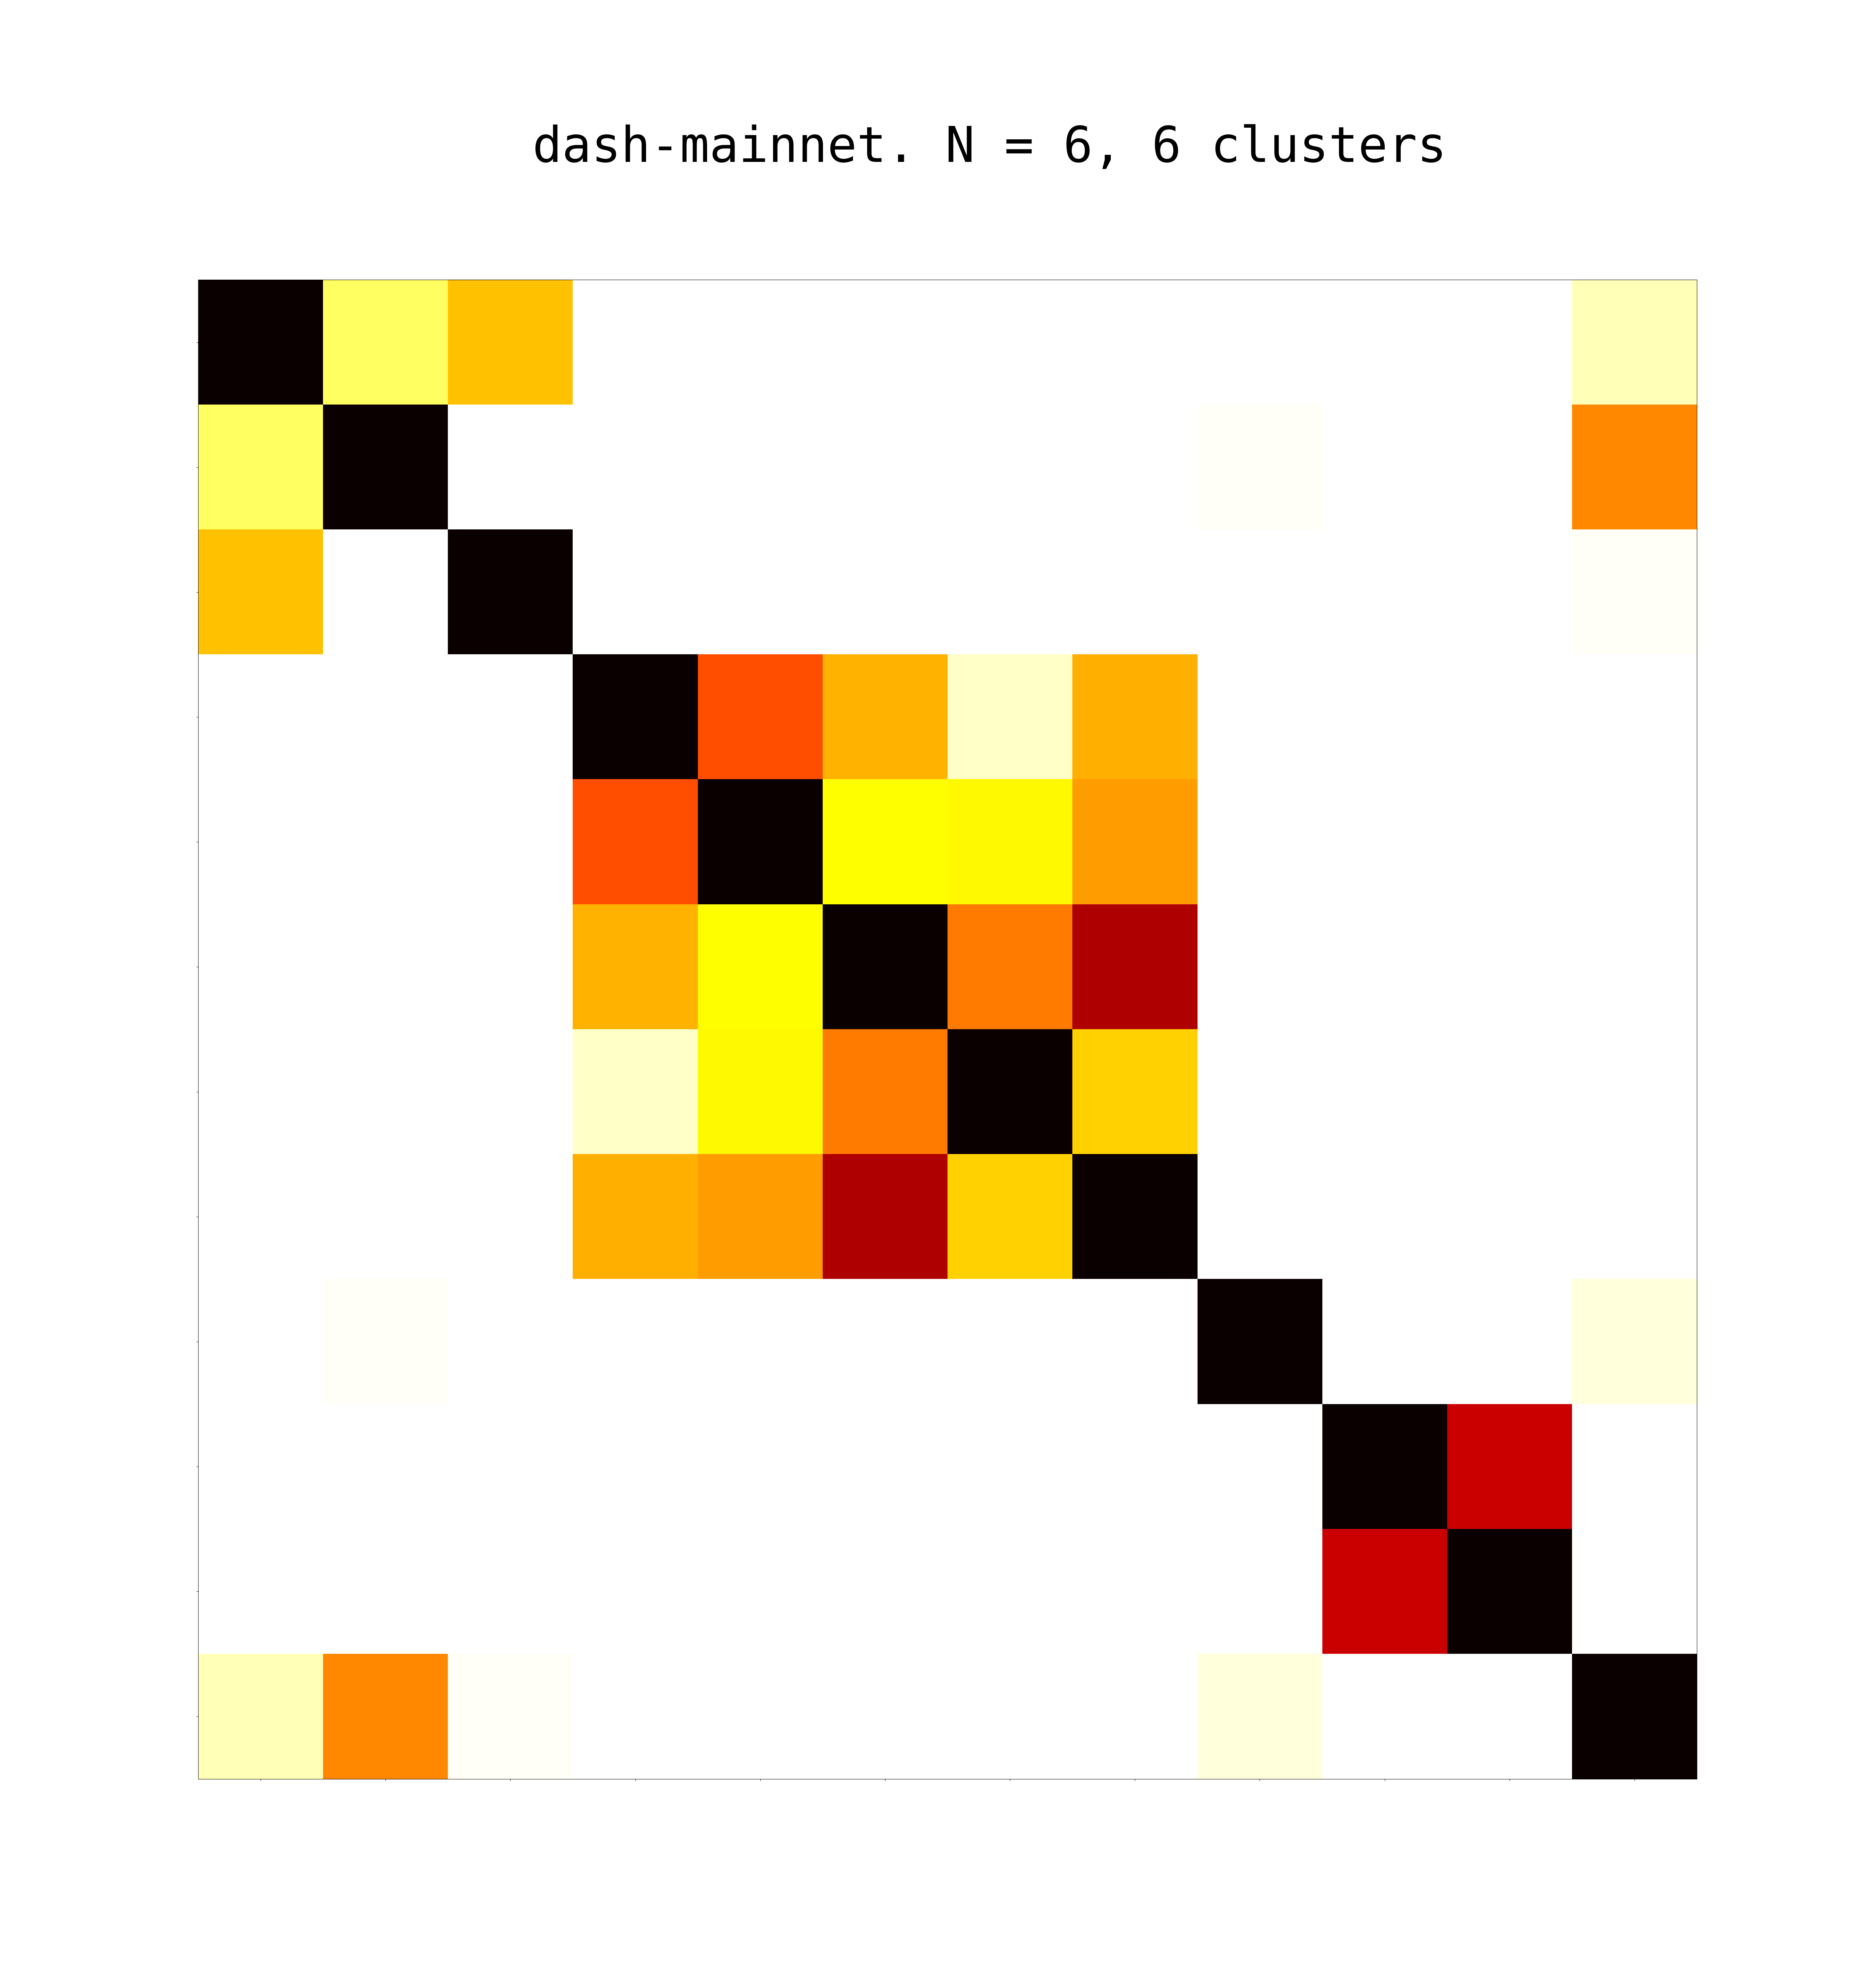
\includegraphics[width=\columnwidth]{dash-mainnet-1531510768.png}
		\caption{Transaction clustering for Dash (transactions only).}
		\label{fig:dash-tx}
	\end{minipage}\hfill
\end{figure*}

We ran our clustering algorithm two times: accounting for the Dash-specific messages (Figure~\ref{fig:dash-all}), and considering only standard transaction inventory messages (Figure~\ref{fig:dash-tx}).
In both cases, we obtained clearly visible clusters.
These preliminary results demonstrate a clear privacy concern, especially if combined with transaction graph analysis~\cite{Kalodner2017}. 


\subsubsection{Monero}

Monero is a privacy-focused cryptocurrency that is not based on the Bitcoin~Core codebase.
Monero provides privacy by default.
Users do not have to explicitly choose the "private" option (such as a shielded address in Zcash and PrivateSend in Dash).

The Monero community recognized the threat of deanonymization through network analysis~\cite{user36432017, manontheinside2016, expez2016, Cameron2016}.
This motivated the integration of Dandelion++ networking protocol in 2020~\cite{ErCiccione2020} (see Section~\ref{sec:Dandelion}).
The Kovri project~\cite{Kovri} aims to add an I2P router into Monero (not deployed as of 2020).
At the time of our experiments (mid-2018), Monero did not use any broadcast randomization technique.
%Monero nodes do not limit the number of incoming connections by default~\cite{user363032016}.

Unlike Bitcoin, Monero does not allow spending a transaction output in the same block it is created in.
A new output appears as "locked" until the transaction that creates it receives $10$~confirmations ($20$~minutes at the target block time of~$2$~minutes)~\cite{dpzz2017}.
Though this is a wallet-level restriction and not a protocol-level one, the major implementations (the official desktop wallet and Monerujo wallet for Android) enforce it.
This means that the scenario of our previous experiments is rather unrealistic.
For example, in order to issue $20$~transactions within a $20$~minute period, a user must have $20$~"unlocked" transaction outputs (each of which takes $20$~minutes to create).

We checked the suitability of our technique on Monero by performing an experiment without our own transactions.
The goal of the experiment was to check if the correlation matrix between transaction weight vectors exhibits a block-diagonal structure.
We connected to $200$~nodes and received $124$~transactions in a $38$~minute window (see Figure~\ref{fig:monero}).

\begin{figure}[!t]
	\centering
	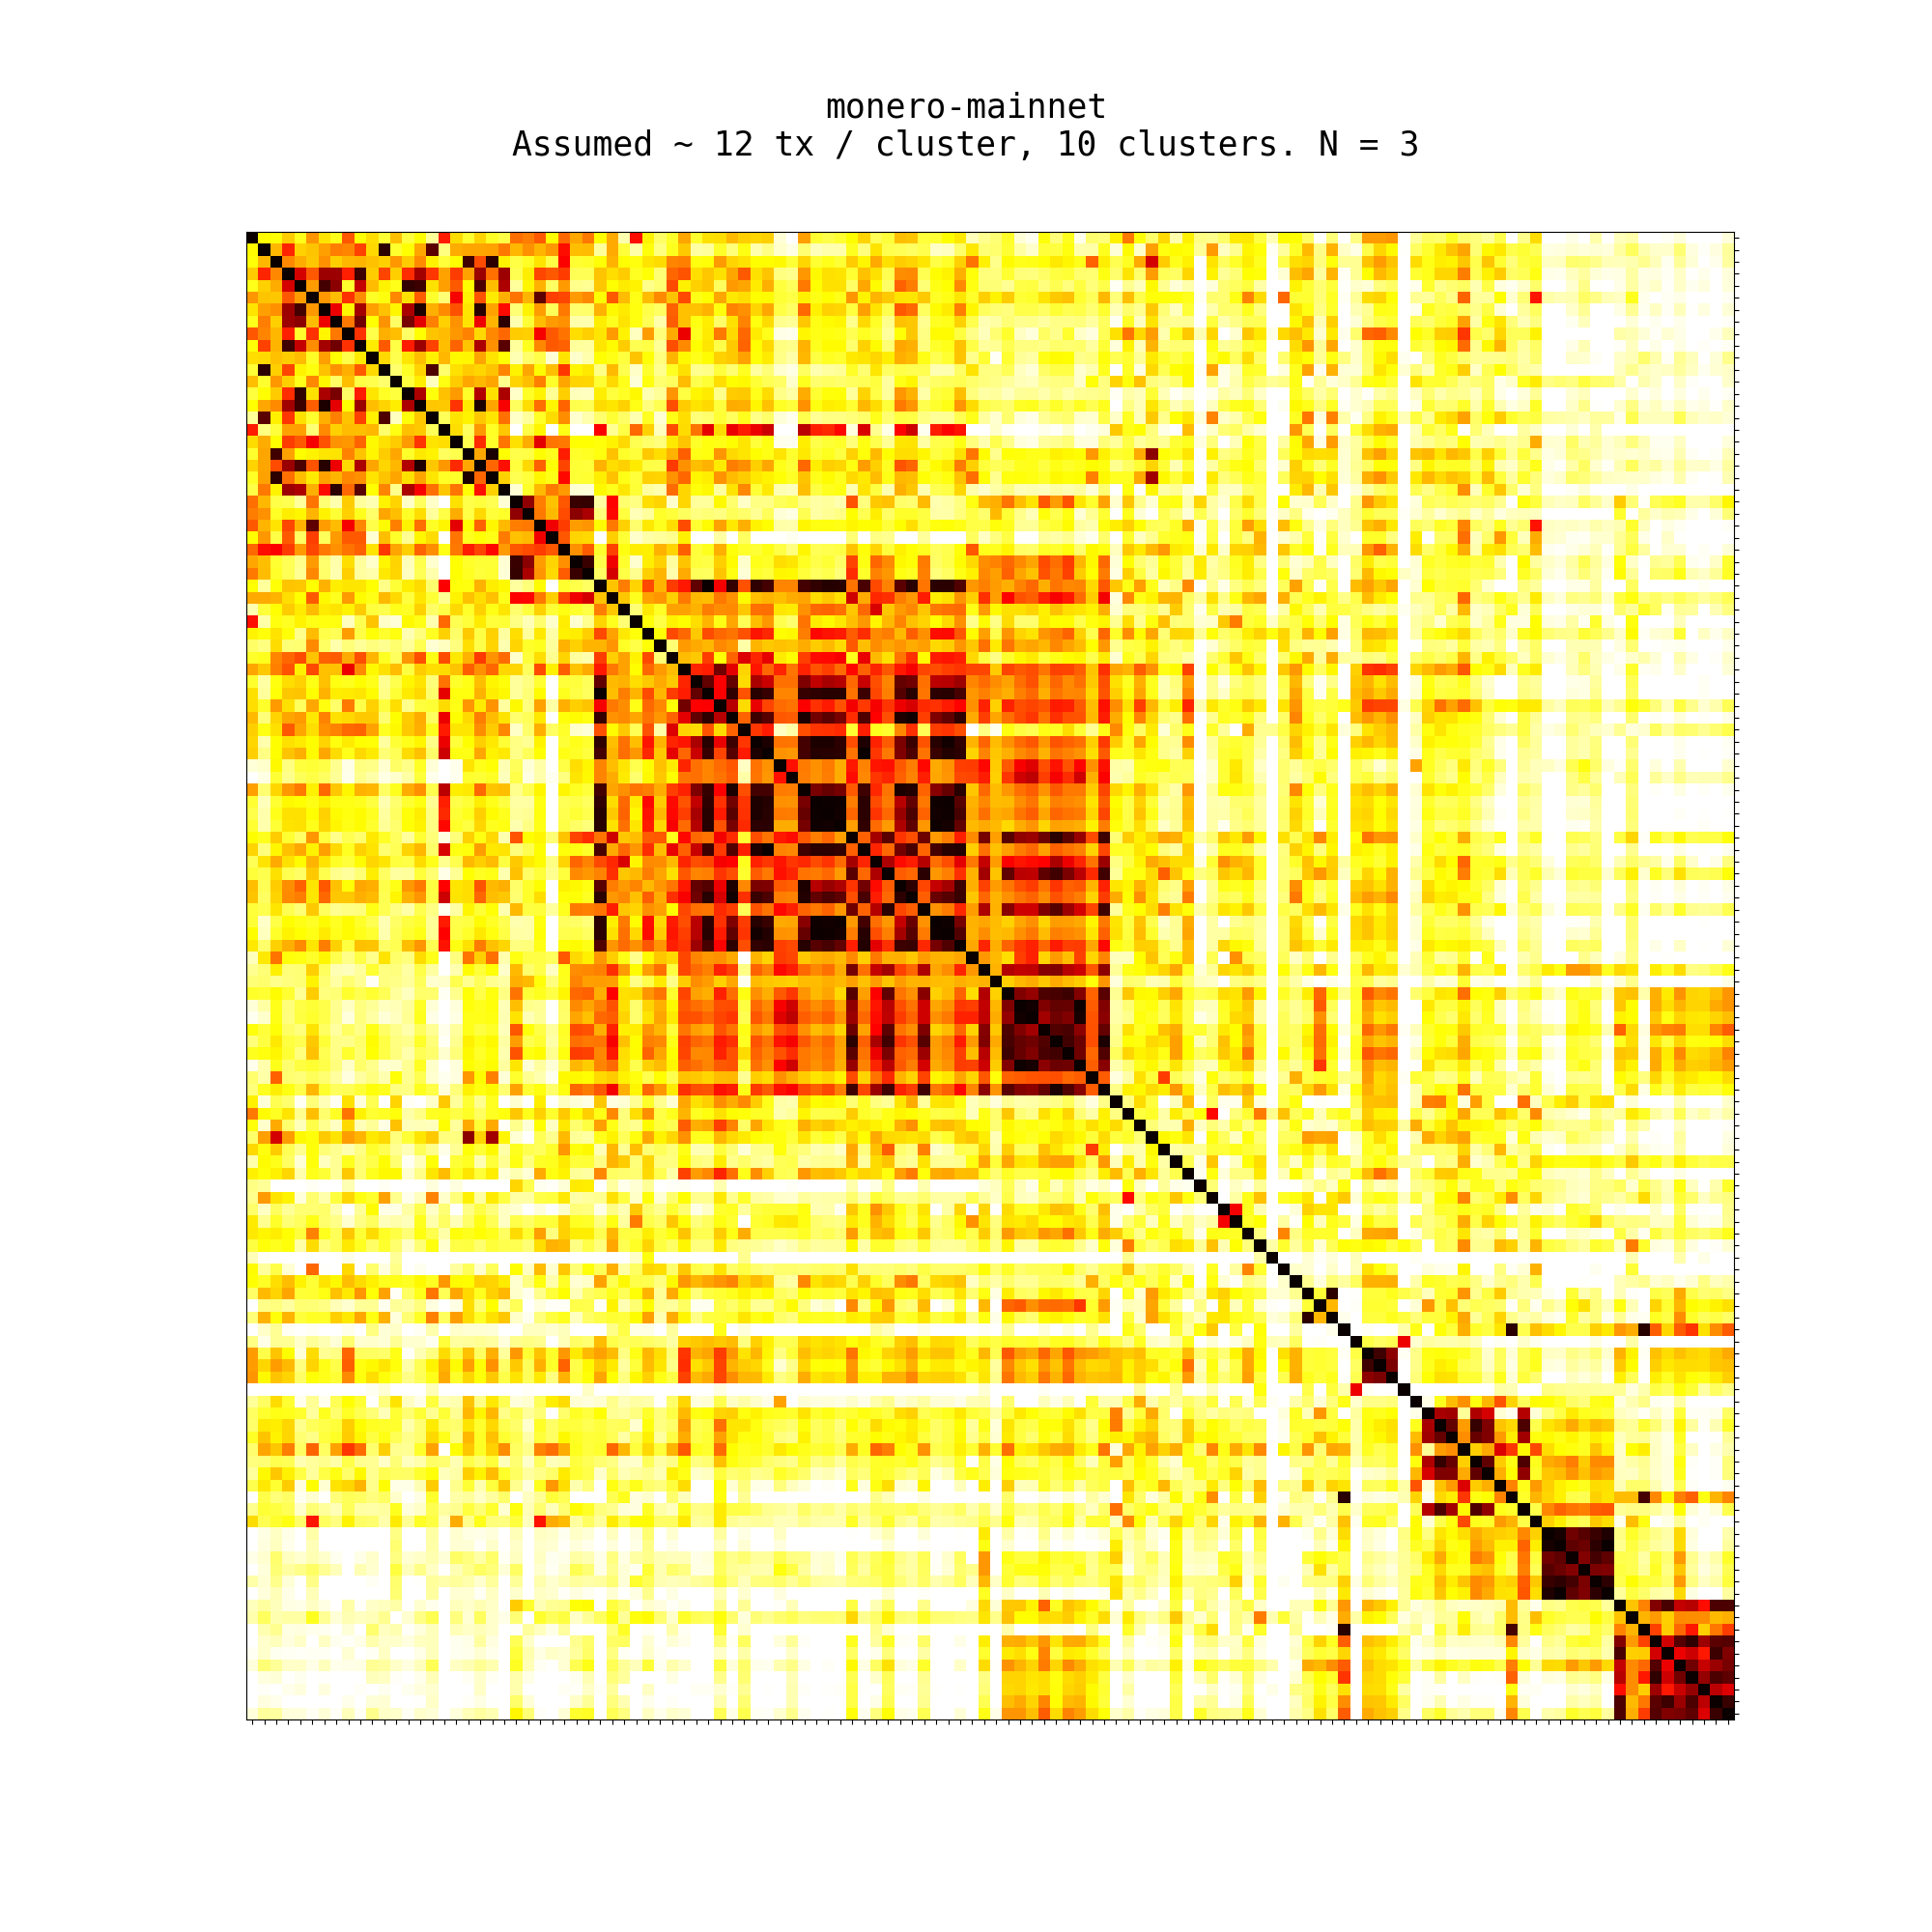
\includegraphics[width=0.5\columnwidth]{monero-mainnet-005-fig-correlations-012-txcl-003-N-Rand-best.png}
	\caption{Transaction clustering for Monero.}
	\label{fig:monero}
\end{figure}

The less clear picture compared to Bitcoin testnet may be explained as follows.
First, we connected to a subset of all nodes (the total number of nodes at the time of the experiment was estimated at $1700$--$1800$~\cite{MoneroHash}).
Second, Monero does not employ the three-step transaction propagation as Bitcoin does.
There is no \texttt{inv} -- \texttt{getdata} -- \texttt{tx} exchange.
This may have had opposite effects on clustering quality.
On the one hand, transactions are relayed unconditionally to all neighbors.
This increases the probability that we receive a new transaction from a node other than the source of one of its entry nodes.
On the other hand, this broadcast type may provide a near-perfect insight into transaction sources, if the attacker connects to all or nearly all nodes.
Third, \texttt{monerod} connects to nodes relatively slowly (compared to \texttt{bcclient}).
In our experiment, while trying to connect to $200$~nodes, we obtained $150$~connections only after approximately $2$~hours, $175$~connections after $3$~hours, $200$~connections after nearly $8$~hours.
This factor made our experiment more difficult.

Monero uses hard-coded DNS seeds and seed IP addresses for bootstrapping (similar to Bitcoin, see Chapter~\ref{sec:BitcoinP2PProtocol}).
As of July~2018, none of the DNS seeds resolves.
The official client falls back to seed IP addresses.


\subsection{Results for mobile wallets}

We also performed analogous experiments on Bitcoin (testnet and mainnet) and Zcash issuing transactions from selected mobile wallets for Android.\footnote{Chapter~\ref{Chapter04Wallets} evaluates other privacy-related aspects of mobile cryptocurrency wallets.}

Most wallets connect to the P2P network indirectly via a trusted server maintained by the wallet's developers.
We refer to wallets that connect to the P2P network directly as \textit{P2P wallets}.
Most P2P wallets rely on the BitcoinJ library for networking.
None of them uses broadcast randomization.
Unlike Bitcoin~Core, BitcoinJ sends \texttt{tx} unconditionally\footnote{Note that in this case a full node receiving a \texttt{tx} message from an SPV node can be sure that the transaction originated at that SPV node, whereas receiving an \texttt{inv} announcement from a full node may also be a re-broadcast. This demonstrates the privacy enhancement of exclusively connecting to a trusted node for SPV.}.
The BitcoinJ developers acknowledge that the three-step \texttt{inv} -- \texttt{getdata} -- \texttt{tx} exchange in Bitcoin~Core improves privacy, but argue that since BitcoinJ is used by SPV nodes with a weaker privacy model, the three-step broadcast would only decrease efficiency.

We chose a diverse selection of wallets for our experiments: Bitcoin-only and multi-coin, with centralized as well as P2P networking.
We performed experiments on Bitcoin testnet (Bitcoin wallet), Bitcoin mainnet (Bitcoin wallet, BRD, Coinomi, Mycelium), and Zcash (Coinomi).
Bitcoin wallet and BRD\footnote{Bitcoin wallet and BRD are the two most popular Bitcoin clients~\cite{Wang2017}.} use P2P broadcast; Coinomi and Mycelium use centralized broadcast.
For wallets with centralized broadcast, we only issue one set of transactions, using it as a "label" for a presumed wallet cluster.
If our transactions form a visible cluster, we inspect the IP addresses of nodes which were among the first ones to broadcast them.
Thus we infer the IP addresses of nodes that are likely to be used for transaction broadcasts for this wallet.
This allows us to later associate transactions in the network with popular wallets.

\begin{figure}
	\centering
	\begin{subfigure}{.5\textwidth}
		\centering
		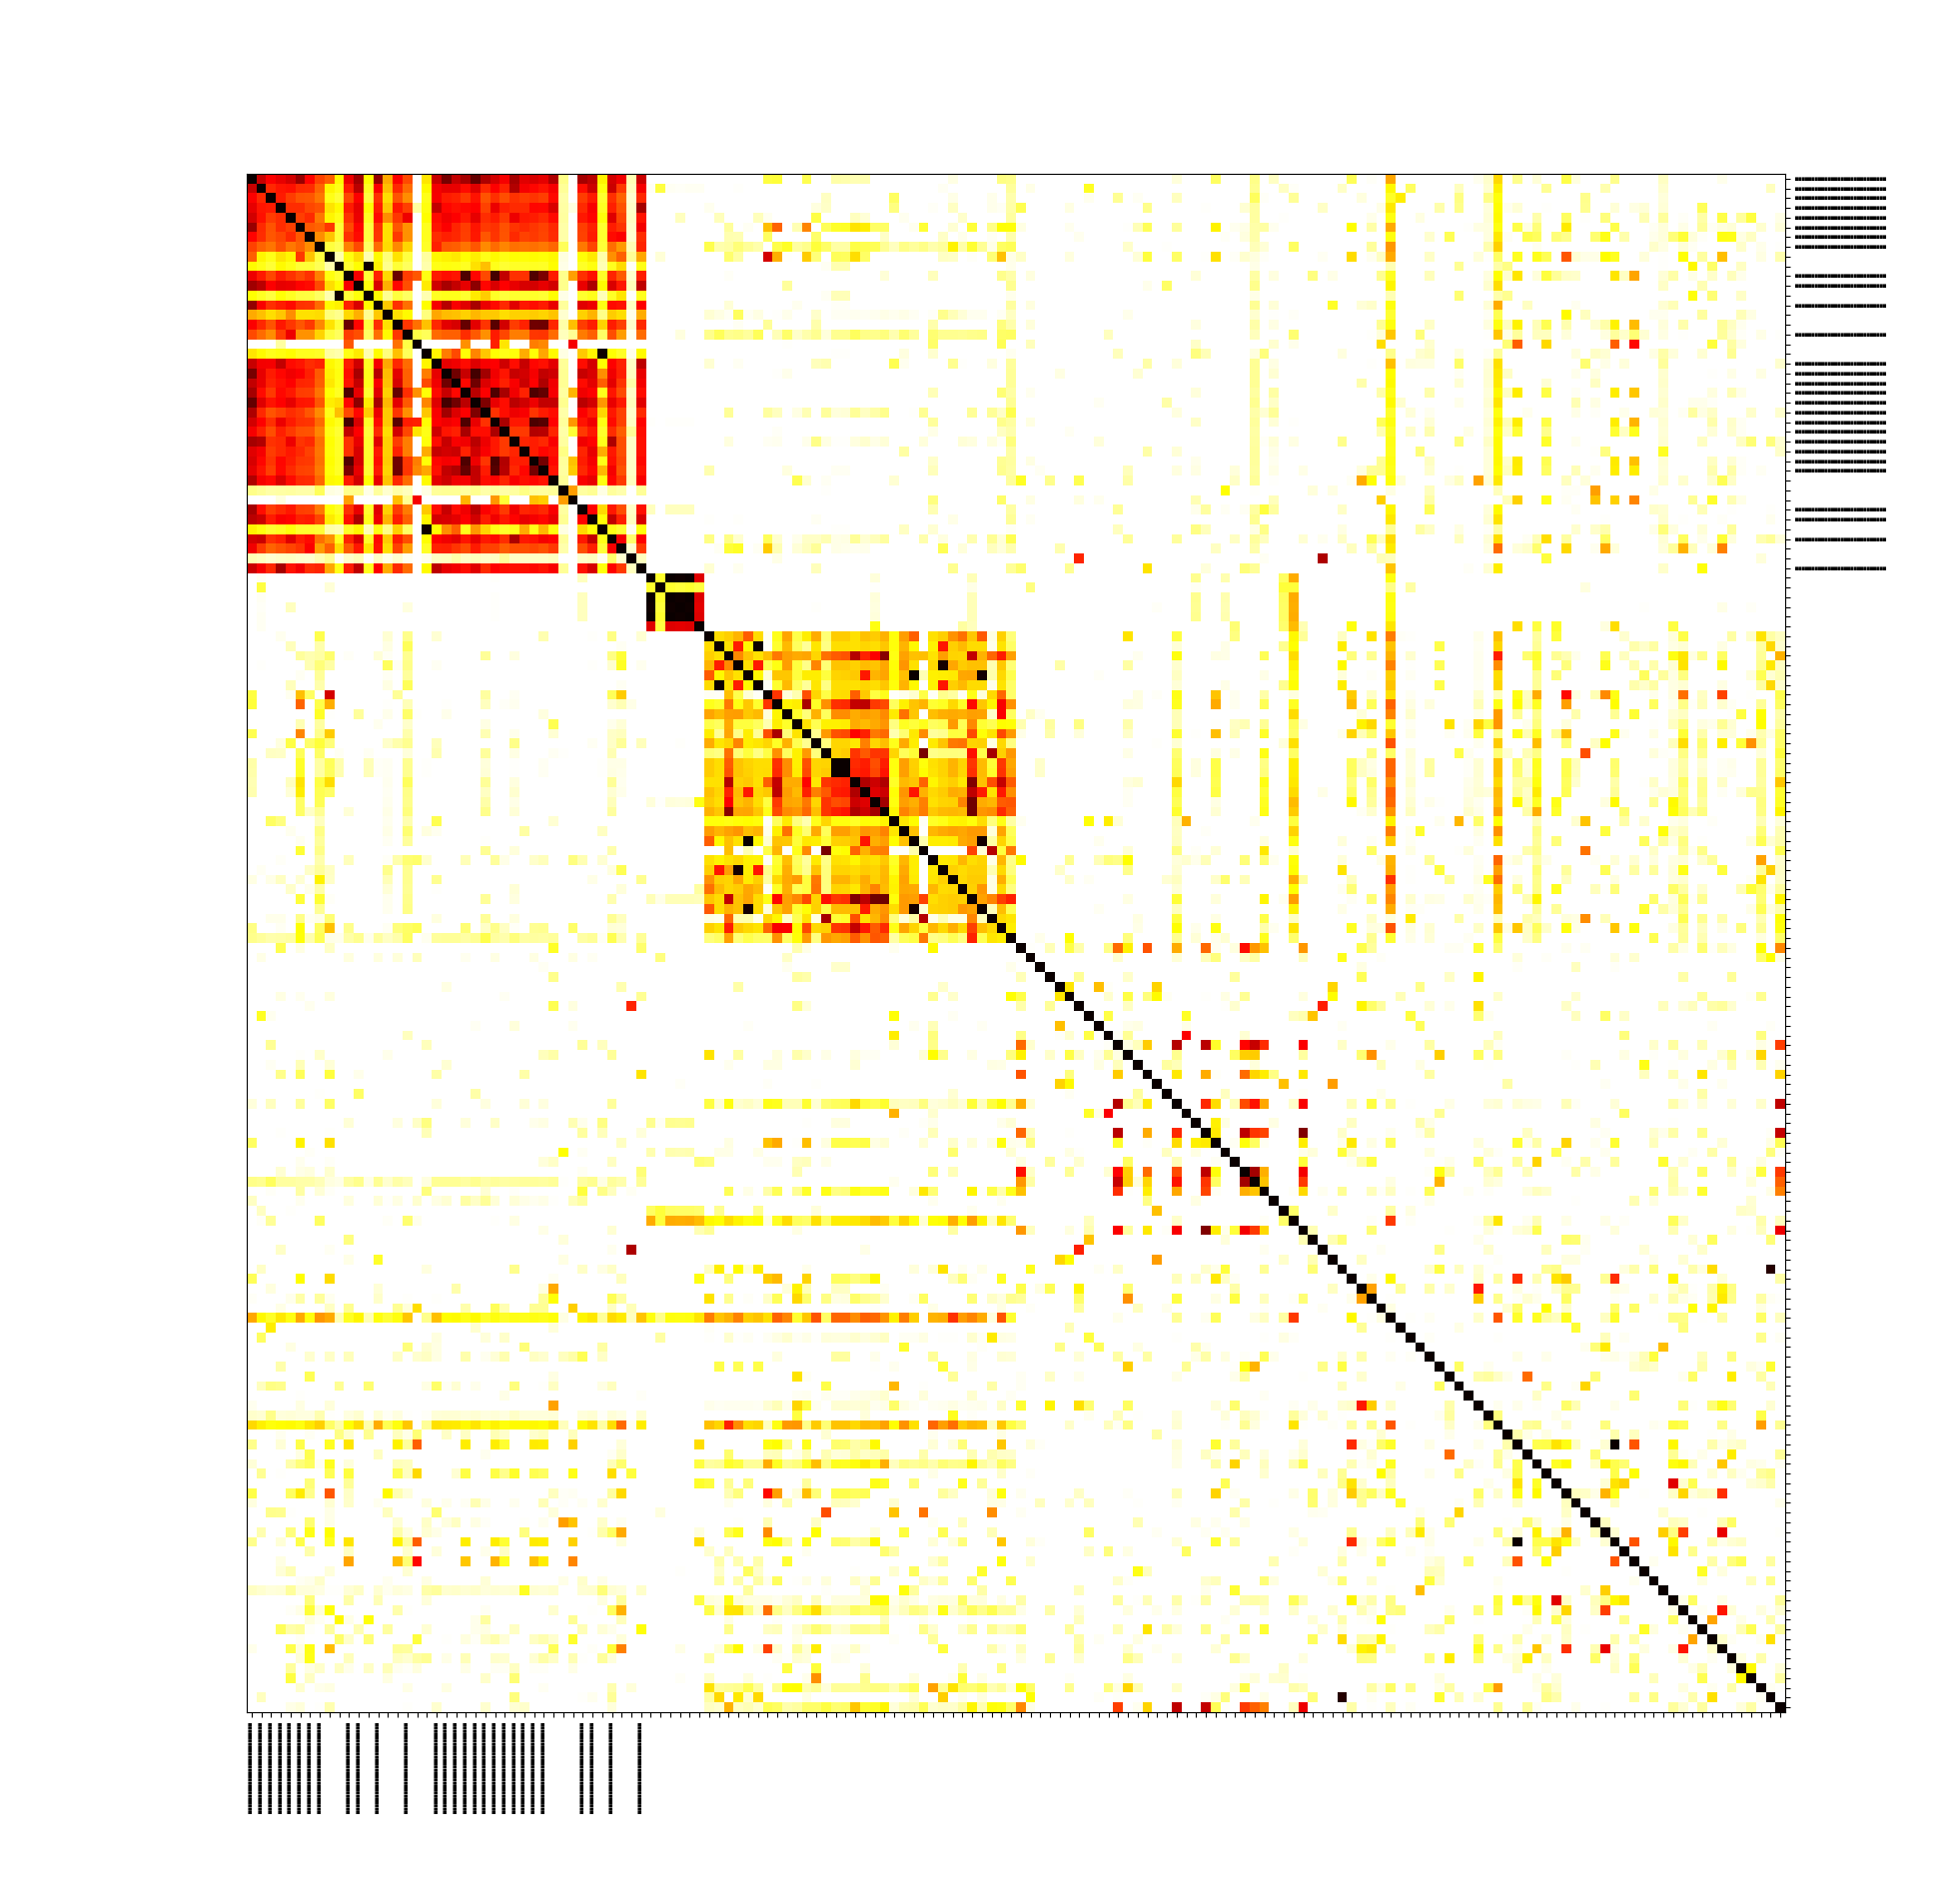
\includegraphics[width=\columnwidth]{bitcoin-testnet-1542895555-fig-corr-032-txcl-005-N-Rand.png}
		\caption{Bitcoin testnet, Mycelium.}
	\end{subfigure}%
	\begin{subfigure}{.5\textwidth}
		\centering
		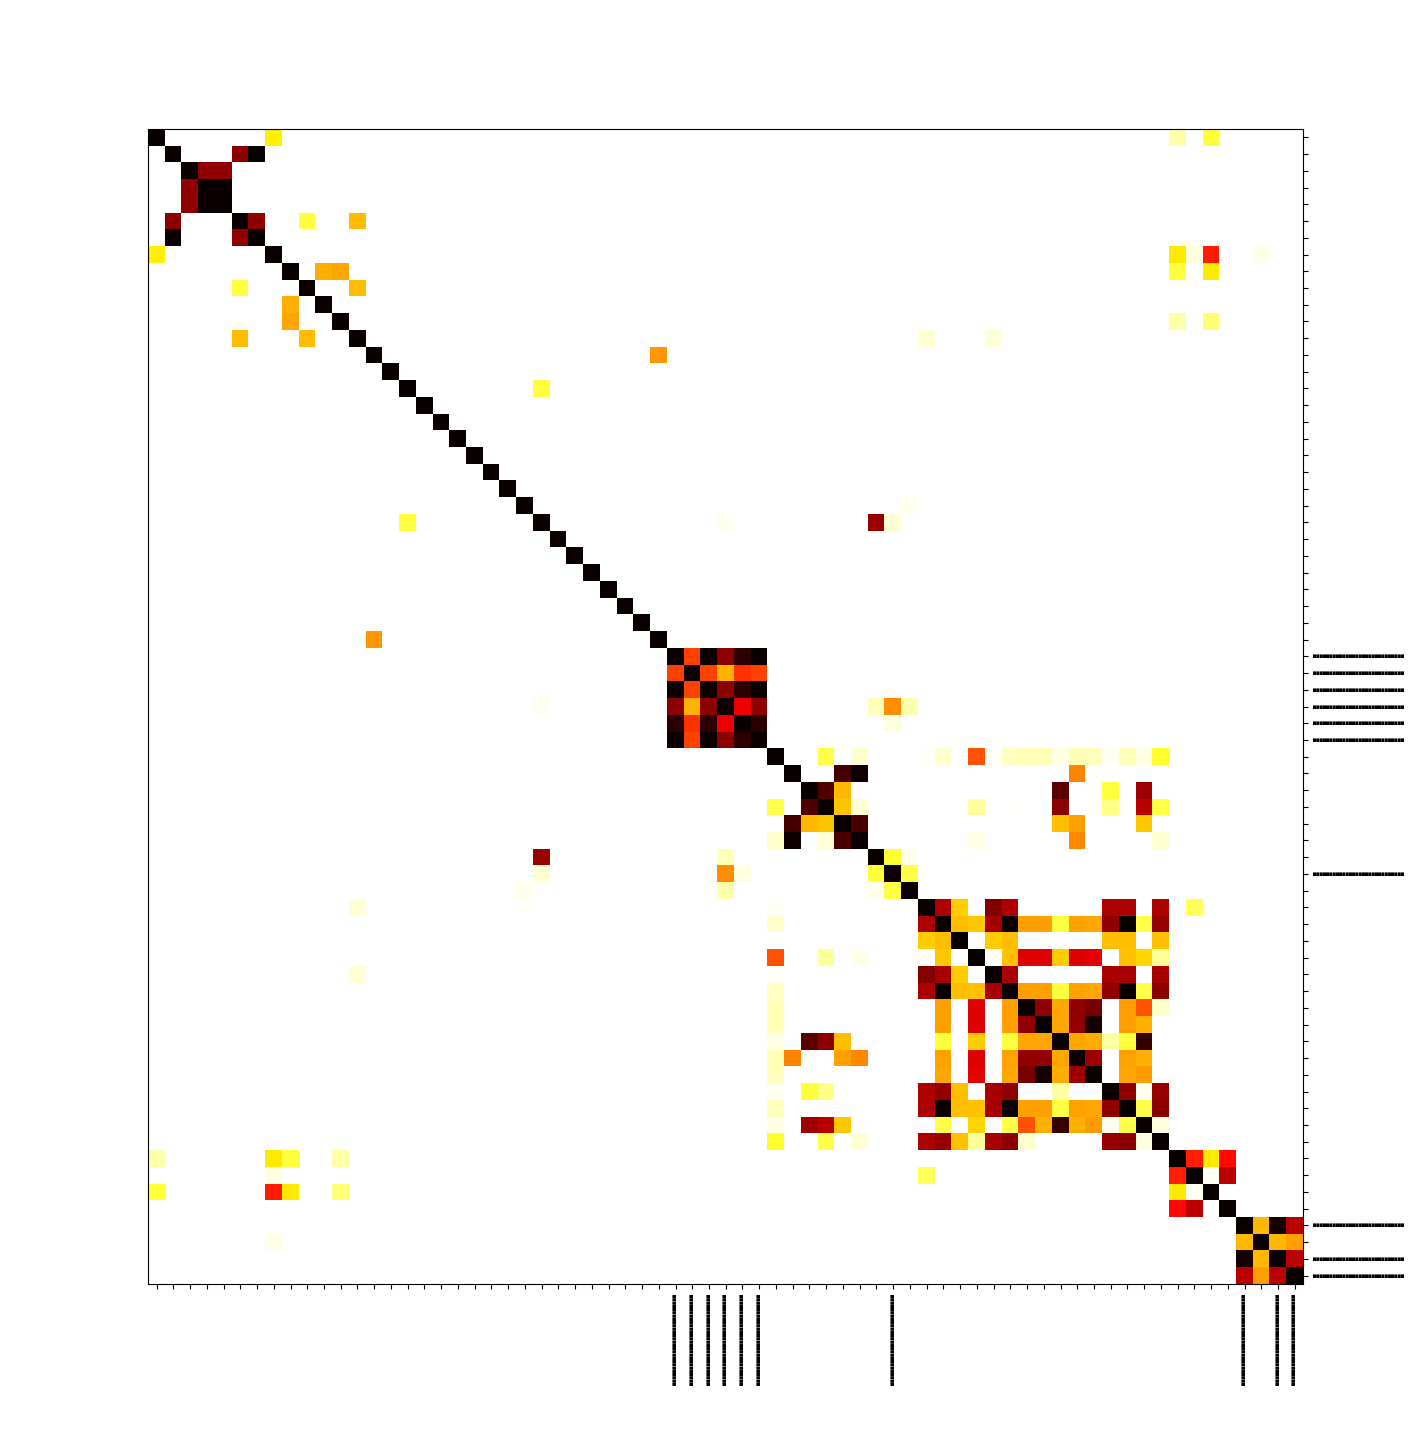
\includegraphics[width=\columnwidth]{bitcoin-testnet-1537202356-fig-corr-008-txcl-003-N-Rand.png}
		\caption{Bitcoin testnet, Bitcoin wallet.}
	\end{subfigure}
	\begin{subfigure}{.5\textwidth}
		\centering
		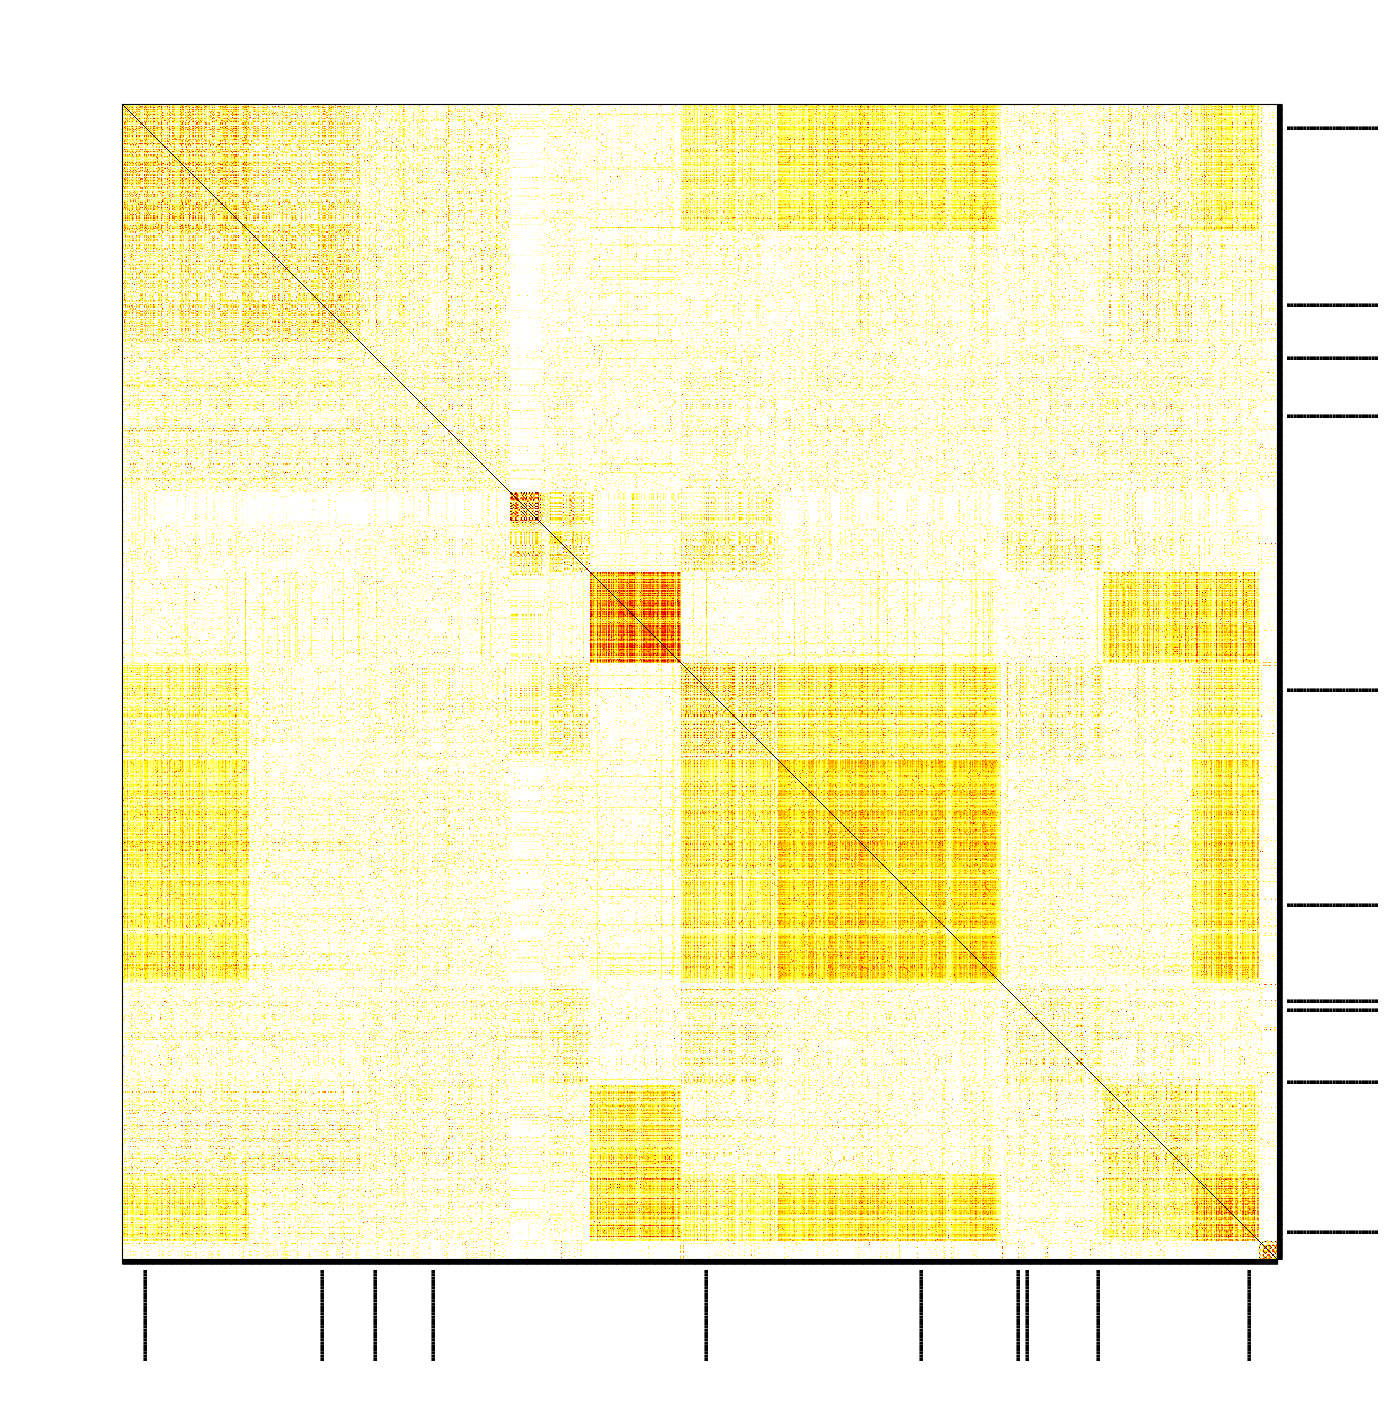
\includegraphics[width=\columnwidth]{bitcoin-mainnet-1537365306-fig-corr-202-txcl-007-N-Rand.png}
		\caption{Bitcoin mainnet, Bitcoin wallet.}
	\end{subfigure}%
	\begin{subfigure}{.5\textwidth}
		\centering
		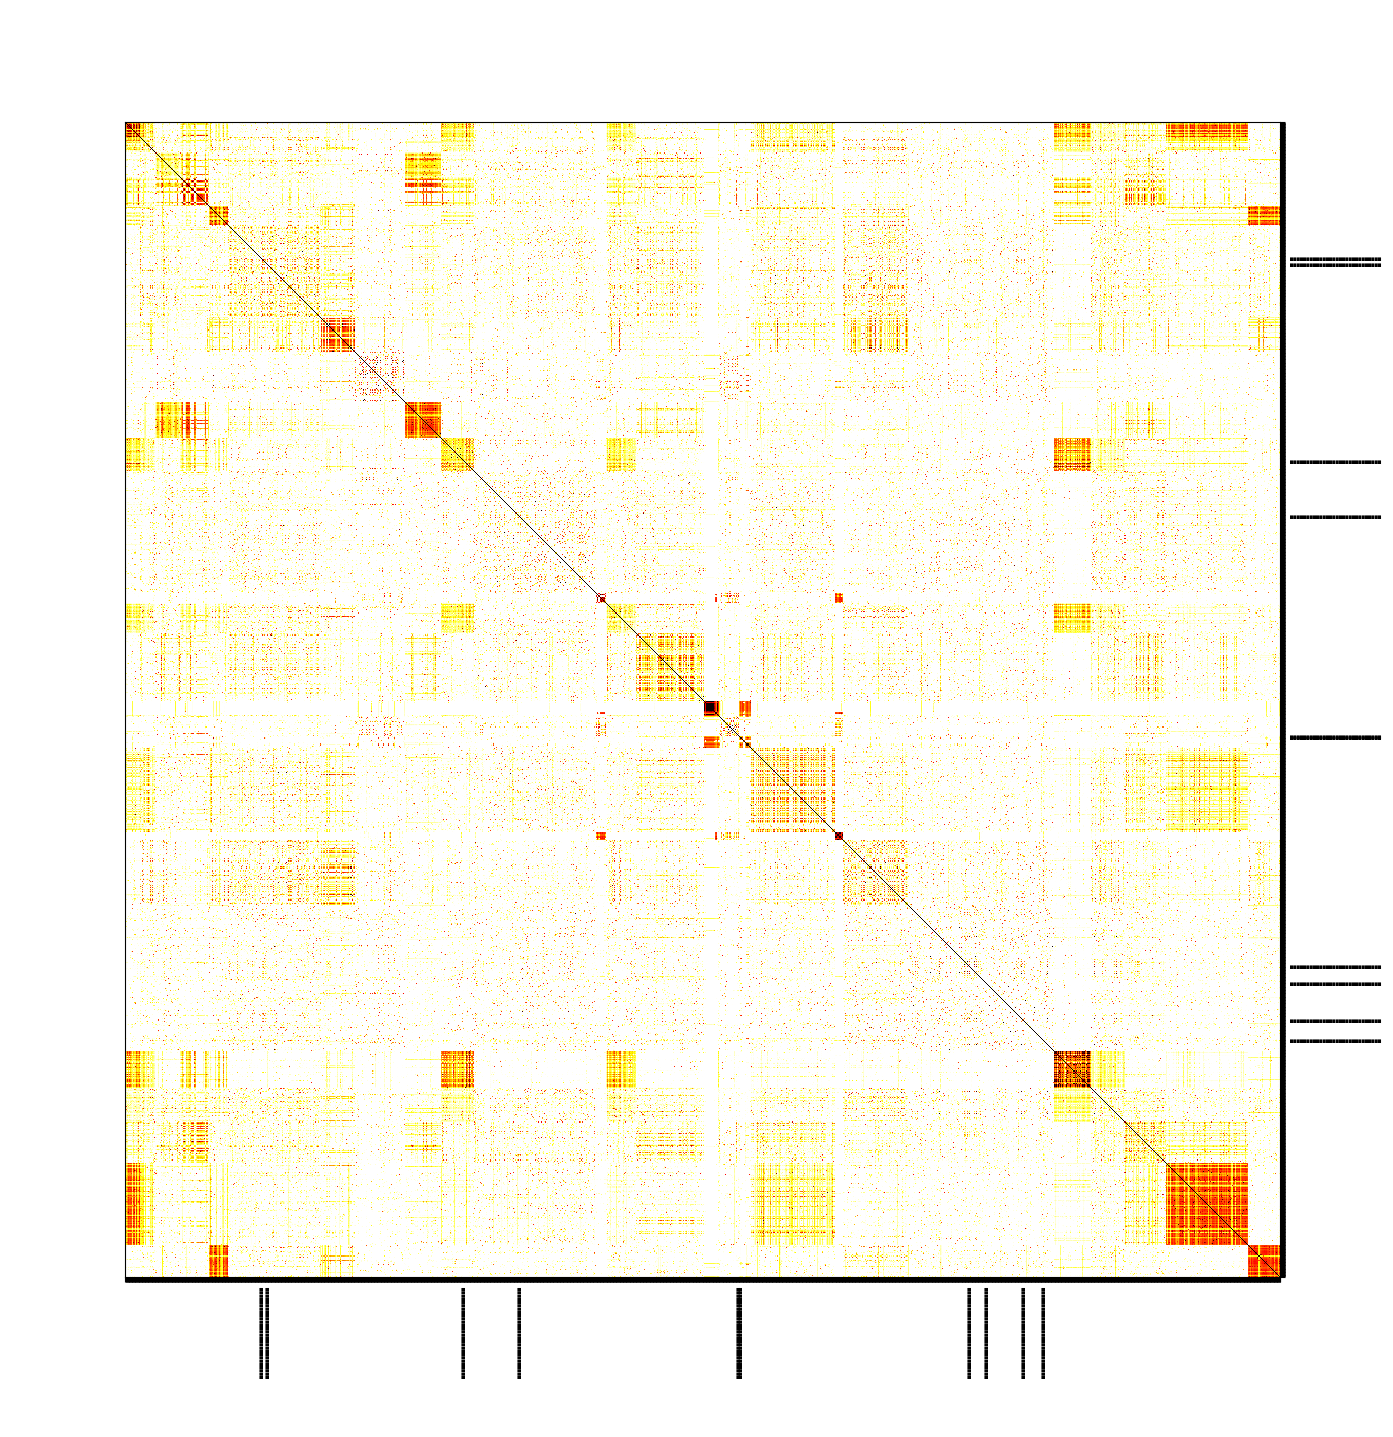
\includegraphics[width=\columnwidth]{bitcoin-mainnet-1537377559-fig-corr-102-txcl-004-N-Rand.png}
		\caption{Bitcoin mainnet, BRD.}
	\end{subfigure}
	\begin{subfigure}{.5\textwidth}
		\centering
		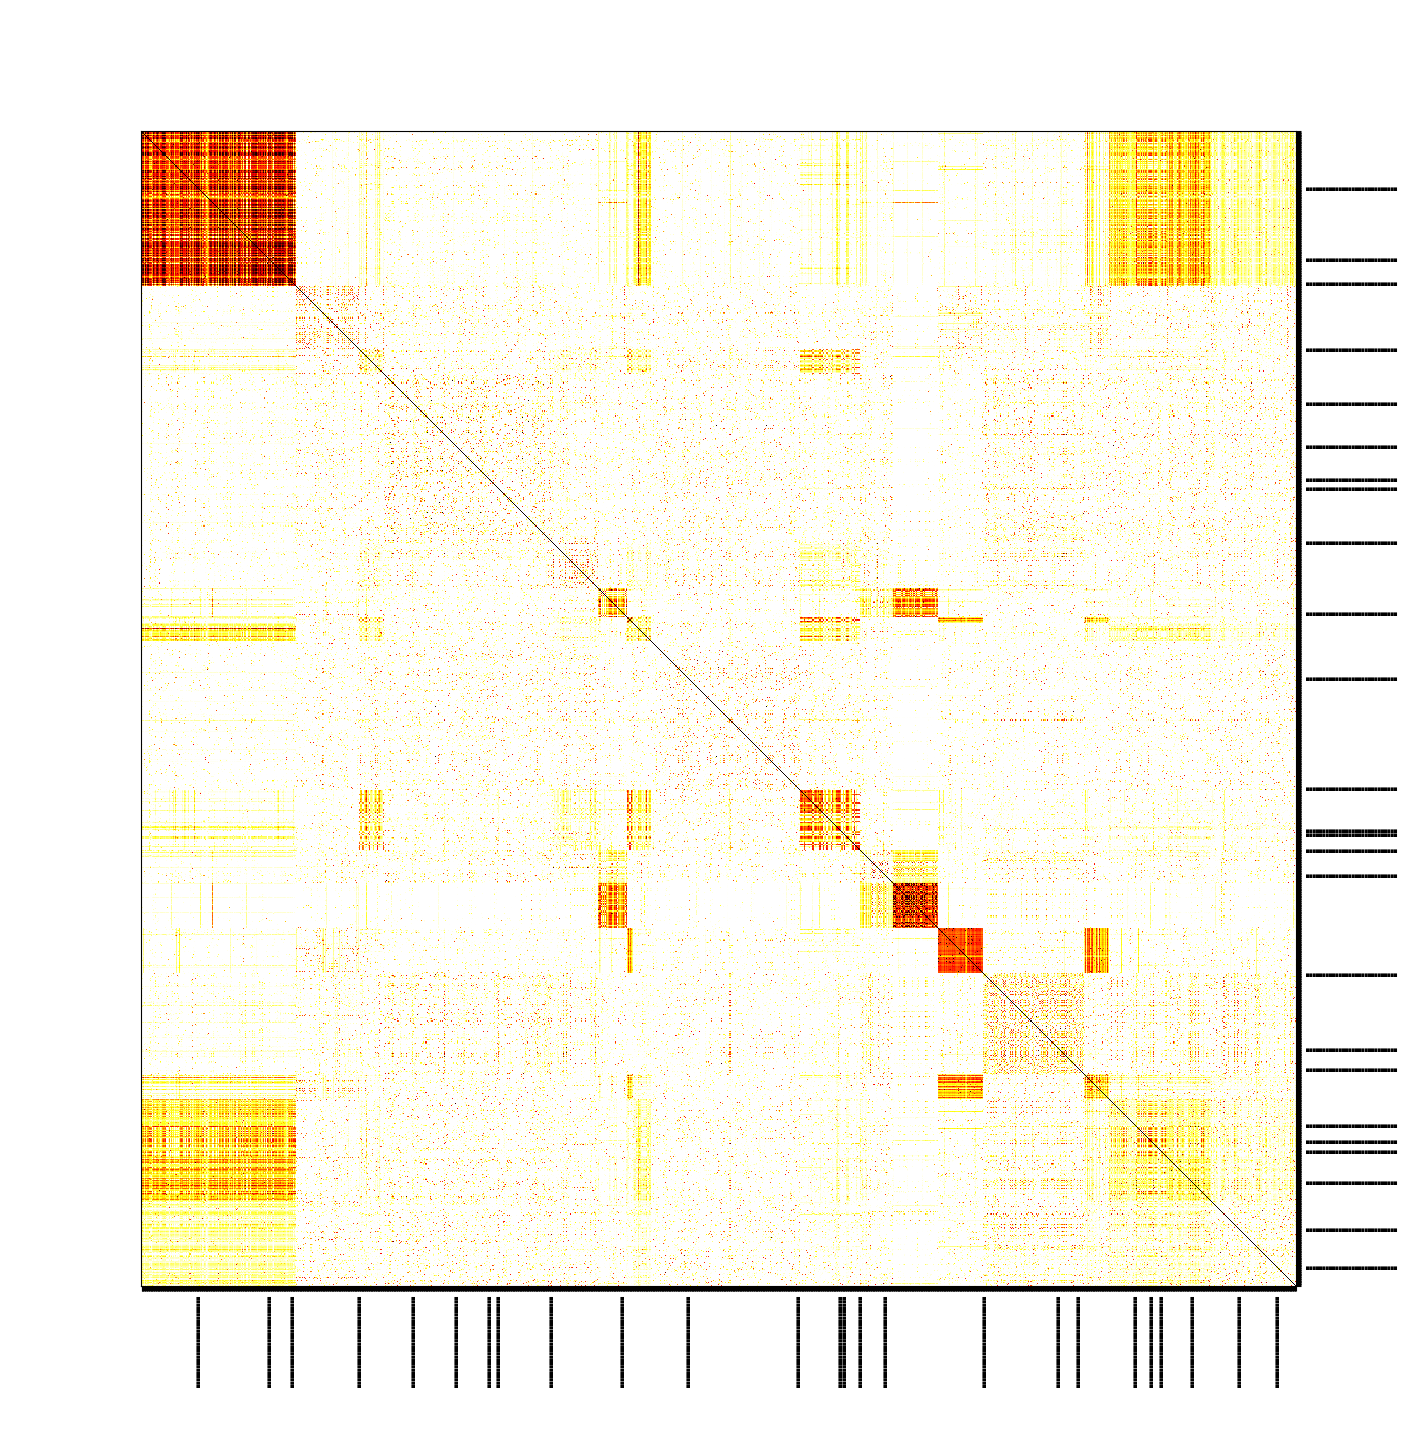
\includegraphics[width=\columnwidth]{bitcoin-mainnet-1537951300-fig-corr-100-txcl-004-N-Rand.png}
		\caption{Bitcoin mainnet, Coinomi.}
	\end{subfigure}%
	\begin{subfigure}{.5\textwidth}
		\centering
		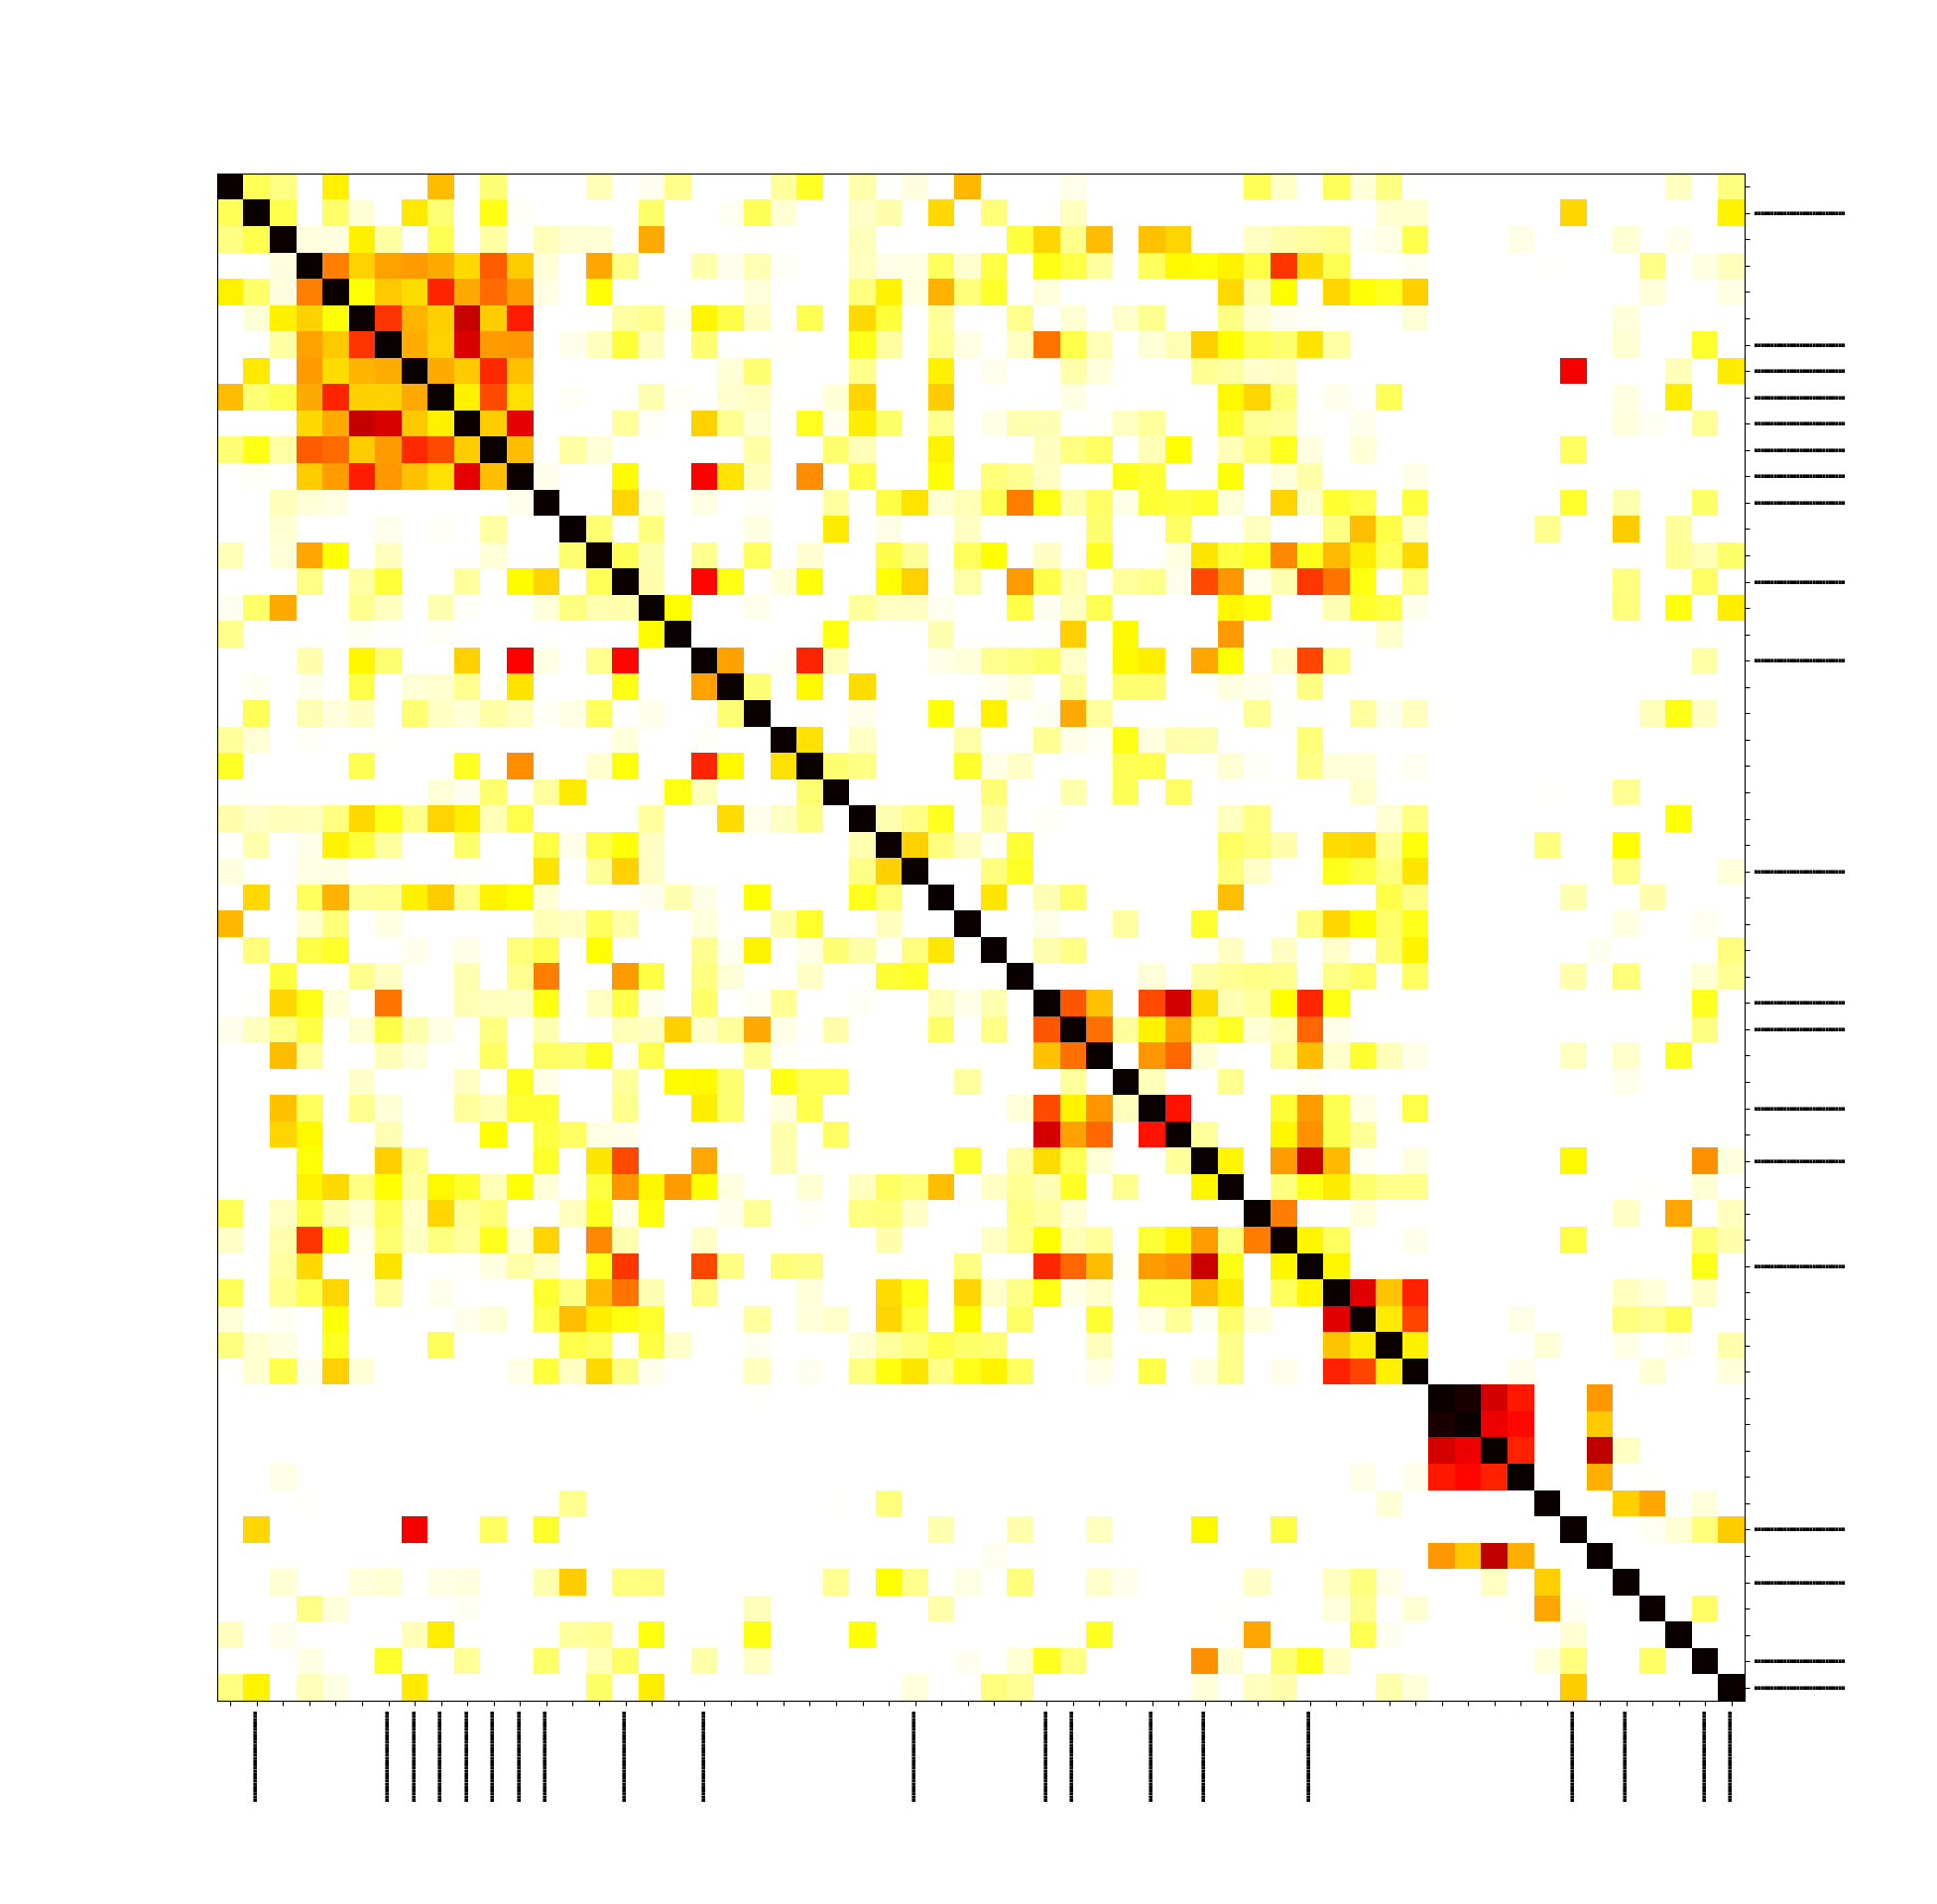
\includegraphics[width=\columnwidth]{zcash-mainnet-1543922496-fig-corr-005-txcl-003-N-Rand.png}
		\caption{Zcash, Coinomi.}
	\end{subfigure}
	\caption{Transaction clustering for mobile wallets.}
	\label{fig:clustering-all}
\end{figure}

The results are presented in Figure~\ref{fig:clustering-all}.
Our control transactions are marked with black ticks.
As expected, the matrices exhibit a block-diagonal structure.
The clusters are clearly visible for the testnet version of Bitcoin wallet, for which we obtained a low (good for the attacker) anonymity degree of~$0.5089$.
The adjusted anonymity degree ($d_{adj}$) for the Bitcoin mainnet is $0.8646$~for Bitcoin wallet, $0.8413$~for BRD, and~$0.9117$~for Coinomi.
While our technique performs well on testnet, the picture for the Bitcoin mainnet is much less clear.
This may be explained by a much larger total number of nodes and transactions, and to the fact that we only run the experiment on a subset of Bitcoin nodes to avoid disrupting the network.


\subsubsection*{Estimating the IP addresses of wallet's nodes}

Apart from clustering transactions, an adversary might be interested in obtaining the IP address of the nodes which a centralized wallet uses for transaction broadcast.
The IP address of a centralized wallet's node may not necessarily be secret.
Still, linking Bitcoin transactions with IP addresses may reveal which wallet a victim is using.
This information can later be leveraged for social engineering attacks.

We test this attack scenario in two experiments.
The first experiment considered Bitcoin testnet and Mycelium wallet.
Mycelium transactions exhibit a clearly visible cluster.
They are quickly propagated from the same two IP addresses.
The time difference between these announcements is in single milliseconds.
Other nodes re-broadcast then only after tens or hundreds of milliseconds.
According to IP geolocation services, the two nodes are located in Germany (\texttt{2a01:4f9:2b:4ca::2}) and in Helsinki, Finland (\texttt{95.216.68.181}).
According to a reverse DNS lookup service \url{robtex.com}, one of these IP addresses corresponds to a URL~\url{electrumx-b.mycelium.com}.
Both IP addresses belong to Hetzner (a cloud provider) and a latency of~$25$~ms~\cite{Bitnodes}.
In a separate experiment, we discovered that there are also Bitcoin mainnet nodes running at the same IP addresses.
Each of them offers more than $700$~connection slots.

The second experiment considered Zcash and Coinomi wallet.
Though our transactions did not form a clear cluster, we observe that some of them (in the second cluster) were first received from the same IP (\texttt{5.79.123.194}), which, we assume, is one of the Coinomi's nodes.


\section{Attack cost estimation}

We now estimate the resources required for a full-scale attack on the Bitcoin mainnet.
The Bitcoin mainnet consists of approximately $10\,000$~nodes reachable at any given time~\cite{Bitnodes}.
% 9887 90-day avg as of 2018-11-11
% https://bitnodes.earn.com/dashboard/?days=90
We estimate Bitcoin nodes to provide $43$~connections slots on average (measured on $1000$~random nodes).
According to~\cite{BitcoinWiki}, the size of an \texttt{inv} message is "36x + const for message with x objects".
We assume that an \texttt{inv} for a single transaction requires $40$~bytes.
As on November~2018, Bitcoin processes around $250\,000$~transactions per day, or $2.89$~transactions per second.
Assuming each connection eventually relays each transaction, we arrive at the required bandwidth for one connection slot as: $2.89 \times 40 = 115.6$~B/s.
A full-scale attack on Bitcoin mainnet would require maintaining an average of~$43$~connections to $10\,000$~nodes, i.e.,~a total bandwidth of~$115.6 \times 10\,000 \times 43 = 49\,708\,000$~B/s = $47.4$~MB/s = $379$~Mbit/s.
An hour-long attack at this bandwidth will require receiving approximately $167$~GB of incoming traffic.

We may estimate the monetary cost of the attack based on the costs of running a Bitcoin full node on a cloud server.
Various estimations put that cost at between $3$~and~$20$~US~dollars per month~\cite{Zeyde2018, Connell2017}.
By default, Bitcoin nodes relay transactions through $8$~outgoing connections and accepts up to $117$~incoming connections.\footnote{The experiments were performed before Bitcoin~Core introduced two additional connections for block propagation. In any case, blocks are outside of the scope of our technique~\cite{Daftuar2019}.}
Assuming an average node has a total of~$125$~slots, $125 - 43 = 82$~slots eventually get occupied.
An adversary needs to maintain $10\,000 \times 43 = 430\,000$~connections, or approximately $5\,244$~times more than a regular node.
Considering that one month ($30$-days) is $720$~hours, we conclude that an estimated cost of an hour-long attack is approximately $5244 \div 720 = 7.3$~times the monthly cost of running a regular full node.
That leads to an estimation of bandwidth costs between $20$~and~$150$~USD\@.
Even taking into account the cost of computation and storage, the total cost of the attack is on the order of hundreds of US~dollars -- well within reach of even amateur adversaries, not to mention professional black-hat hackers and nation states.

All our experiments on Bitcoin testnet and Zcash mainnet cost $35$~USD\@.
This can likely be decreased by optimizing the scripts, storing data locally, etc.


\section{Discussion and countermeasures}

Our technique performs well on relatively small network and works to some extent on Bitcoin.
We expect a more resourceful attacker to achieve better results by establishing more connections to more Bitcoin nodes.
The main limitation is the assumption that a user issues multiple transactions during a relatively short time frame through the same node.

Application-level cryptographic countermeasures, such as zero-knowledge proofs in Zcash, can not defend against our attack.
We only consider transaction hashes and their announcement times, ignoring their content.

A popular mitigation for deanonymization attacks are overlay networks such as Tor~\cite{Tor}.
In our case, these countermeasures may not be efficient.
From the point of view of our method, transactions announced from the same Bitcoin node would form a cluster, even if they were sent to this node through Tor.
Moreover, broadcasting transactions via Tor may even introduce additional man-in-the-middle vulnerabilities~\cite{Biryukov2015}.

Practical countermeasures depend on the type of the wallet.

For a full node that accepts incoming connections (a server):

\begin{itemize}
	\item Run the node with an increased number of outgoing connections to dilute the quality of the topological fingerprint;
	\item Use additional random delays on top of those implemented in the node software;
	\item Drop connections to randomly chosen entry nodes and establish new ones, constantly altering the set of entry nodes;
	\item Give advice to users not to broadcast sensitive transactions within a short period of time (if the server is used for broadcasting transactions of multiple users).
\end{itemize}

Users of full nodes without incoming connections (for example, behind NAT) may wish to re-launch the software after making a transaction, so that each transaction is broadcast through a new set of entry nodes.

Proposed countermeasures for SPV nodes would be:

\begin{itemize}
	\item Use wallets with P2P broadcast (e.g.,~Bitcoin wallet for Android~\cite{BitcoinWallet});
	\item If using wallets with centralized broadcast, use different wallets for transactions that are not meant to be linkable;
	\item connect to a trusted full node.
\end{itemize}

All users should avoid sending multiple transactions within a short time frame.

Note that an attacker may leverage additional information to increase clustering accuracy, such as known addresses of exchanges and other service providers~\cite{Walletexplorer}.

\paragraph{Dandelion}
Dandelion is a P2P protocol for cryptocurrencies (see~Section~\ref{sec:Dandelion}) that is an effective countermeasure against our attack.\footnote{The authors mention (\cite{Fanti2018}, Section~4.2) that some configurations of the protocol may be prone to transaction correlation attacks.}
The key property of the current P2P protocols that we exploit is that nodes do not distinguish between incoming and outgoing connections.
Transactions are propagated to a random subset picked from all connections.
This allow a well-connected listener to receive more information by initiating more connections.
For instance, by saturating $50\%$~of a node's connection slots, a listener has a $50\%$~chance to be the first to receive a new transaction from it.

In Dandelion, nodes choose neighbors for the stem phase only from their outgoing connections.
An attacker has no easy way to force a remote peer to initiate a connection.
Therefore, a malicious node with many outgoing connections does not have any advantage in the stem phase.
It can only aggregate incoming information while acting as a regular relay, which may gain some but not much insight into possible transaction clusters.


\section{Conclusion} \label{sec:Ch03Conclusion}

We have studied the state of anonymity of cryptocurrencies on the network level.
We have described and implemented a novel transaction clustering method based on the analysis of transaction announcements.
We have implemented and tested our technique on four popular cryptocurrencies using a variety of wallets.

Our results indicate that Bitcoin and the major privacy-focused cryptocurrencies do not sufficiently defend against our attack.
A low budget adversary can accurately link transactions that have been broadcast from the same node.
Additionally, a similar technique allows an attacker to infer the IP addresses of nodes used for transaction broadcast by certain mobile wallets.
Cryptocurrencies should defend against network analysis to provide stronger privacy guarantees.
